% Options for packages loaded elsewhere
\PassOptionsToPackage{unicode}{hyperref}
\PassOptionsToPackage{hyphens}{url}
\PassOptionsToPackage{dvipsnames,svgnames,x11names}{xcolor}
%
\documentclass[
  letterpaper,
  DIV=11,
  numbers=noendperiod]{scrartcl}

\usepackage{amsmath,amssymb}
\usepackage{iftex}
\ifPDFTeX
  \usepackage[T1]{fontenc}
  \usepackage[utf8]{inputenc}
  \usepackage{textcomp} % provide euro and other symbols
\else % if luatex or xetex
  \usepackage{unicode-math}
  \defaultfontfeatures{Scale=MatchLowercase}
  \defaultfontfeatures[\rmfamily]{Ligatures=TeX,Scale=1}
\fi
\usepackage{lmodern}
\ifPDFTeX\else  
    % xetex/luatex font selection
\fi
% Use upquote if available, for straight quotes in verbatim environments
\IfFileExists{upquote.sty}{\usepackage{upquote}}{}
\IfFileExists{microtype.sty}{% use microtype if available
  \usepackage[]{microtype}
  \UseMicrotypeSet[protrusion]{basicmath} % disable protrusion for tt fonts
}{}
\makeatletter
\@ifundefined{KOMAClassName}{% if non-KOMA class
  \IfFileExists{parskip.sty}{%
    \usepackage{parskip}
  }{% else
    \setlength{\parindent}{0pt}
    \setlength{\parskip}{6pt plus 2pt minus 1pt}}
}{% if KOMA class
  \KOMAoptions{parskip=half}}
\makeatother
\usepackage{xcolor}
\setlength{\emergencystretch}{3em} % prevent overfull lines
\setcounter{secnumdepth}{-\maxdimen} % remove section numbering
% Make \paragraph and \subparagraph free-standing
\makeatletter
\ifx\paragraph\undefined\else
  \let\oldparagraph\paragraph
  \renewcommand{\paragraph}{
    \@ifstar
      \xxxParagraphStar
      \xxxParagraphNoStar
  }
  \newcommand{\xxxParagraphStar}[1]{\oldparagraph*{#1}\mbox{}}
  \newcommand{\xxxParagraphNoStar}[1]{\oldparagraph{#1}\mbox{}}
\fi
\ifx\subparagraph\undefined\else
  \let\oldsubparagraph\subparagraph
  \renewcommand{\subparagraph}{
    \@ifstar
      \xxxSubParagraphStar
      \xxxSubParagraphNoStar
  }
  \newcommand{\xxxSubParagraphStar}[1]{\oldsubparagraph*{#1}\mbox{}}
  \newcommand{\xxxSubParagraphNoStar}[1]{\oldsubparagraph{#1}\mbox{}}
\fi
\makeatother

\usepackage{color}
\usepackage{fancyvrb}
\newcommand{\VerbBar}{|}
\newcommand{\VERB}{\Verb[commandchars=\\\{\}]}
\DefineVerbatimEnvironment{Highlighting}{Verbatim}{commandchars=\\\{\}}
% Add ',fontsize=\small' for more characters per line
\usepackage{framed}
\definecolor{shadecolor}{RGB}{241,243,245}
\newenvironment{Shaded}{\begin{snugshade}}{\end{snugshade}}
\newcommand{\AlertTok}[1]{\textcolor[rgb]{0.68,0.00,0.00}{#1}}
\newcommand{\AnnotationTok}[1]{\textcolor[rgb]{0.37,0.37,0.37}{#1}}
\newcommand{\AttributeTok}[1]{\textcolor[rgb]{0.40,0.45,0.13}{#1}}
\newcommand{\BaseNTok}[1]{\textcolor[rgb]{0.68,0.00,0.00}{#1}}
\newcommand{\BuiltInTok}[1]{\textcolor[rgb]{0.00,0.23,0.31}{#1}}
\newcommand{\CharTok}[1]{\textcolor[rgb]{0.13,0.47,0.30}{#1}}
\newcommand{\CommentTok}[1]{\textcolor[rgb]{0.37,0.37,0.37}{#1}}
\newcommand{\CommentVarTok}[1]{\textcolor[rgb]{0.37,0.37,0.37}{\textit{#1}}}
\newcommand{\ConstantTok}[1]{\textcolor[rgb]{0.56,0.35,0.01}{#1}}
\newcommand{\ControlFlowTok}[1]{\textcolor[rgb]{0.00,0.23,0.31}{\textbf{#1}}}
\newcommand{\DataTypeTok}[1]{\textcolor[rgb]{0.68,0.00,0.00}{#1}}
\newcommand{\DecValTok}[1]{\textcolor[rgb]{0.68,0.00,0.00}{#1}}
\newcommand{\DocumentationTok}[1]{\textcolor[rgb]{0.37,0.37,0.37}{\textit{#1}}}
\newcommand{\ErrorTok}[1]{\textcolor[rgb]{0.68,0.00,0.00}{#1}}
\newcommand{\ExtensionTok}[1]{\textcolor[rgb]{0.00,0.23,0.31}{#1}}
\newcommand{\FloatTok}[1]{\textcolor[rgb]{0.68,0.00,0.00}{#1}}
\newcommand{\FunctionTok}[1]{\textcolor[rgb]{0.28,0.35,0.67}{#1}}
\newcommand{\ImportTok}[1]{\textcolor[rgb]{0.00,0.46,0.62}{#1}}
\newcommand{\InformationTok}[1]{\textcolor[rgb]{0.37,0.37,0.37}{#1}}
\newcommand{\KeywordTok}[1]{\textcolor[rgb]{0.00,0.23,0.31}{\textbf{#1}}}
\newcommand{\NormalTok}[1]{\textcolor[rgb]{0.00,0.23,0.31}{#1}}
\newcommand{\OperatorTok}[1]{\textcolor[rgb]{0.37,0.37,0.37}{#1}}
\newcommand{\OtherTok}[1]{\textcolor[rgb]{0.00,0.23,0.31}{#1}}
\newcommand{\PreprocessorTok}[1]{\textcolor[rgb]{0.68,0.00,0.00}{#1}}
\newcommand{\RegionMarkerTok}[1]{\textcolor[rgb]{0.00,0.23,0.31}{#1}}
\newcommand{\SpecialCharTok}[1]{\textcolor[rgb]{0.37,0.37,0.37}{#1}}
\newcommand{\SpecialStringTok}[1]{\textcolor[rgb]{0.13,0.47,0.30}{#1}}
\newcommand{\StringTok}[1]{\textcolor[rgb]{0.13,0.47,0.30}{#1}}
\newcommand{\VariableTok}[1]{\textcolor[rgb]{0.07,0.07,0.07}{#1}}
\newcommand{\VerbatimStringTok}[1]{\textcolor[rgb]{0.13,0.47,0.30}{#1}}
\newcommand{\WarningTok}[1]{\textcolor[rgb]{0.37,0.37,0.37}{\textit{#1}}}

\providecommand{\tightlist}{%
  \setlength{\itemsep}{0pt}\setlength{\parskip}{0pt}}\usepackage{longtable,booktabs,array}
\usepackage{calc} % for calculating minipage widths
% Correct order of tables after \paragraph or \subparagraph
\usepackage{etoolbox}
\makeatletter
\patchcmd\longtable{\par}{\if@noskipsec\mbox{}\fi\par}{}{}
\makeatother
% Allow footnotes in longtable head/foot
\IfFileExists{footnotehyper.sty}{\usepackage{footnotehyper}}{\usepackage{footnote}}
\makesavenoteenv{longtable}
\usepackage{graphicx}
\makeatletter
\def\maxwidth{\ifdim\Gin@nat@width>\linewidth\linewidth\else\Gin@nat@width\fi}
\def\maxheight{\ifdim\Gin@nat@height>\textheight\textheight\else\Gin@nat@height\fi}
\makeatother
% Scale images if necessary, so that they will not overflow the page
% margins by default, and it is still possible to overwrite the defaults
% using explicit options in \includegraphics[width, height, ...]{}
\setkeys{Gin}{width=\maxwidth,height=\maxheight,keepaspectratio}
% Set default figure placement to htbp
\makeatletter
\def\fps@figure{htbp}
\makeatother

\KOMAoption{captions}{tableheading}
\makeatletter
\@ifpackageloaded{caption}{}{\usepackage{caption}}
\AtBeginDocument{%
\ifdefined\contentsname
  \renewcommand*\contentsname{Table of contents}
\else
  \newcommand\contentsname{Table of contents}
\fi
\ifdefined\listfigurename
  \renewcommand*\listfigurename{List of Figures}
\else
  \newcommand\listfigurename{List of Figures}
\fi
\ifdefined\listtablename
  \renewcommand*\listtablename{List of Tables}
\else
  \newcommand\listtablename{List of Tables}
\fi
\ifdefined\figurename
  \renewcommand*\figurename{Figure}
\else
  \newcommand\figurename{Figure}
\fi
\ifdefined\tablename
  \renewcommand*\tablename{Table}
\else
  \newcommand\tablename{Table}
\fi
}
\@ifpackageloaded{float}{}{\usepackage{float}}
\floatstyle{ruled}
\@ifundefined{c@chapter}{\newfloat{codelisting}{h}{lop}}{\newfloat{codelisting}{h}{lop}[chapter]}
\floatname{codelisting}{Listing}
\newcommand*\listoflistings{\listof{codelisting}{List of Listings}}
\makeatother
\makeatletter
\makeatother
\makeatletter
\@ifpackageloaded{caption}{}{\usepackage{caption}}
\@ifpackageloaded{subcaption}{}{\usepackage{subcaption}}
\makeatother

\ifLuaTeX
  \usepackage{selnolig}  % disable illegal ligatures
\fi
\usepackage{bookmark}

\IfFileExists{xurl.sty}{\usepackage{xurl}}{} % add URL line breaks if available
\urlstyle{same} % disable monospaced font for URLs
\hypersetup{
  pdftitle={Sustainability Goals in Türkiye: Energy, Emissions, and the Future},
  colorlinks=true,
  linkcolor={blue},
  filecolor={Maroon},
  citecolor={Blue},
  urlcolor={Blue},
  pdfcreator={LaTeX via pandoc}}


\title{Sustainability Goals in Türkiye: Energy, Emissions, and the
Future}
\author{}
\date{}

\begin{document}
\maketitle

\renewcommand*\contentsname{Table of contents}
{
\hypersetup{linkcolor=}
\setcounter{tocdepth}{3}
\tableofcontents
}

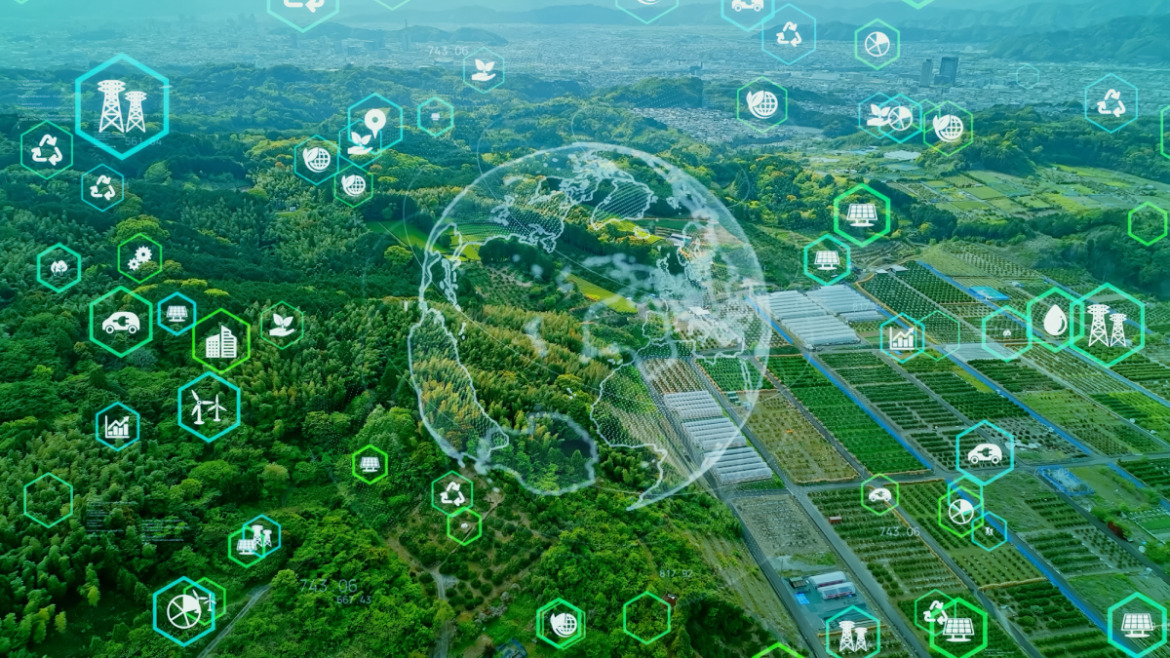
\includegraphics[width=5.77083in,height=\textheight]{images/Energy.jpg}

\section{1. Project Overview and
Scope}\label{project-overview-and-scope}

\begin{quote}
Energy production and consumption are among the primary drivers of
climate change, as they are major sources of carbon emissions. The
continuous rise in energy demand, fueled by economic growth and
industrialization, directly accelerates carbon emissions. In this study,
we aim to investigate the relationship between energy consumption and
carbon emissions originating from the energy sector in Turkey over the
years.

First, correlation and regression analyses will be conducted to reveal
the linear relationship between energy consumption and carbon emissions.
Then, time series analysis will be applied to evaluate the trends of
emissions and energy consumption over the years, the sectoral
distribution of carbon emissions from the energy sector will also be
examined, with a particular focus on emissions from electricity
generation due to its dominant share.\\
Additionally, the relationships between key indicators---such as energy
intensity (primary energy consumption/GDP), per capita energy
consumption, and per capita carbon emissions---will be analyzed to
assess the potential for decoupling carbon emissions from economic
growth.
\end{quote}

\section{2. Data}\label{data}

\subsection{2.1 Data Source}\label{data-source}

\begin{itemize}
\item
  \href{https://data.tuik.gov.tr/Bulten/Index?p=Sera-Gazi-Emisyon-Istatistikleri-1990-2023-53974}{Sera
  Gazı Emisyon İstatistikleri}
\item
  \href{https://data.tuik.gov.tr/Kategori/GetKategori?p=ulusal-hesaplar-113}{Gayri
  Safi Yurtiçi Hasıla ve Kişi Başına Gayri Safi Yurtiçi Hasıla}
\item
  \href{https://www.iea.org/countries/turkiye/energy-mix}{IEA Türkiye
  Enerji İstatistikleri}
\item
  \href{https://www.iea.org/countries/turkiye/emissions}{IEA Enerji
  Kaynaklı Emisyonlar}
\item
  \href{https://www.iea.org/countries/turkiye/electricity}{IEA Elektrik
  Üretim ve Tüketim Verileri}
\item
  \href{https://www.iea.org/countries/turkiye/renewables}{IEA Türkiye
  Yenilenebilir Enerji Kaynakları Verisi}
\end{itemize}

\subsection{2.2 General Information About
Data}\label{general-information-about-data}

The data obtained from TÜİK provide information on the sectoral
distribution of carbon emissions in Türkiye over the years, as well as
GDP figures necessary for calculating energy intensity. Additionally,
the data gathered from the IEA include Türkiye's total primary energy
supply, annual energy amounts by source, energy-related carbon
emissions, the carbon intensity of the energy mix, per capita carbon
emissions, electricity generation and consumption figures, and the share
of renewable energy sources in electricity generation.

\subsection{2.3 Reason of Choice}\label{reason-of-choice}

This study has been selected with the aim of contributing to sustainable
development goals in line with energy and climate policies.\\
In order to shed light on the extent to which carbon-free growth is
achievable and how Turkey's trends over the years align with these
goals, this topic has been chosen from the perspectives of energy,
environment, and society, particularly given that energy-related
emissions constitute a major portion of global warming.\\
Raising awareness on this issue is also one of the primary motivations
behind the study.

\subsection{2.4 Preprocessing}\label{preprocessing}

\href{https://github.com/emu-hacettepe-analytics/emu660-spring2025-NimetSevinc/blob/main/emissions.RData}{Emissions.RData}

\begin{Shaded}
\begin{Highlighting}[]
\FunctionTok{library}\NormalTok{(readr)}
\FunctionTok{library}\NormalTok{(readxl)}
\FunctionTok{library}\NormalTok{(dplyr)}
\FunctionTok{library}\NormalTok{(ggplot2)}
\FunctionTok{library}\NormalTok{(reshape2)}
\FunctionTok{library}\NormalTok{(tidyverse)}
\FunctionTok{library}\NormalTok{(ggthemes)}
\FunctionTok{library}\NormalTok{(knitr)}
\NormalTok{Co2\_emissions\_by\_sector }\OtherTok{\textless{}{-}} \FunctionTok{read\_csv}\NormalTok{(}\StringTok{"C:/Users/DELL/Documents/GitHub/emu660{-}spring2025{-}NimetSevinc/project\_data/International Energy Agency {-} CO2 emissions by sector in Türkiye.csv"}\NormalTok{) }\SpecialCharTok{|\textgreater{}} \FunctionTok{rename}\NormalTok{(}\StringTok{"CO2 emissions by sector"} \OtherTok{=} \StringTok{"CO2 emissions by sector in Türkiye"}\NormalTok{) }\SpecialCharTok{|\textgreater{}} \FunctionTok{select}\NormalTok{(}\SpecialCharTok{{-}}\DecValTok{4}\NormalTok{)}
\FunctionTok{kable}\NormalTok{(}\FunctionTok{head}\NormalTok{(Co2\_emissions\_by\_sector))}
\end{Highlighting}
\end{Shaded}

\begin{longtable}[]{@{}lrr@{}}
\toprule\noalign{}
CO2 emissions by sector & Value & Year \\
\midrule\noalign{}
\endhead
\bottomrule\noalign{}
\endlastfoot
Electricity and heat producers & 68.358 & 2000 \\
Electricity and heat producers & 69.831 & 2001 \\
Electricity and heat producers & 64.531 & 2002 \\
Electricity and heat producers & 65.531 & 2003 \\
Electricity and heat producers & 66.620 & 2004 \\
Electricity and heat producers & 74.515 & 2005 \\
\end{longtable}

\begin{Shaded}
\begin{Highlighting}[]
\FunctionTok{str}\NormalTok{(Co2\_emissions\_by\_sector)}
\end{Highlighting}
\end{Shaded}

\begin{verbatim}
tibble [207 x 3] (S3: tbl_df/tbl/data.frame)
 $ CO2 emissions by sector: chr [1:207] "Electricity and heat producers" "Electricity and heat producers" "Electricity and heat producers" "Electricity and heat producers" ...
 $ Value                  : num [1:207] 68.4 69.8 64.5 65.5 66.6 ...
 $ Year                   : num [1:207] 2000 2001 2002 2003 2004 ...
\end{verbatim}

\begin{Shaded}
\begin{Highlighting}[]
\NormalTok{Co2\_emissions\_fuel\_combustion }\OtherTok{\textless{}{-}} \FunctionTok{read\_csv}\NormalTok{(}\StringTok{"C:/Users/DELL/Documents/GitHub/emu660{-}spring2025{-}NimetSevinc/project\_data/International Energy Agency {-} CO2 emissions from fuel combustion, Türkiye (1).csv"}\NormalTok{) }\SpecialCharTok{|\textgreater{}} \FunctionTok{rename}\NormalTok{(}\StringTok{"CO2 emissions from fuel combustion"} \OtherTok{=} \StringTok{"CO2 emissions from fuel combustion, Türkiye"}\NormalTok{) }\SpecialCharTok{|\textgreater{}} \FunctionTok{select}\NormalTok{(}\SpecialCharTok{{-}}\DecValTok{3}\NormalTok{)}

\FunctionTok{str}\NormalTok{(Co2\_emissions\_fuel\_combustion)}
\end{Highlighting}
\end{Shaded}

\begin{verbatim}
tibble [23 x 2] (S3: tbl_df/tbl/data.frame)
 $ Year                              : num [1:23] 2000 2001 2002 2003 2004 ...
 $ CO2 emissions from fuel combustion: num [1:23] 201 183 193 203 207 ...
\end{verbatim}

\begin{Shaded}
\begin{Highlighting}[]
\NormalTok{Co2\_emissions\_per\_cap }\OtherTok{\textless{}{-}} \FunctionTok{read\_csv}\NormalTok{(}\StringTok{"C:/Users/DELL/Documents/GitHub/emu660{-}spring2025{-}NimetSevinc/project\_data/International Energy Agency {-} CO2 emissions per capita, Türkiye.csv"}\NormalTok{) }\SpecialCharTok{|\textgreater{}} \FunctionTok{rename}\NormalTok{(}\StringTok{"CO2 emissions per capita"} \OtherTok{=} \StringTok{"CO2 emissions per capita, Türkiye"}\NormalTok{) }\SpecialCharTok{|\textgreater{}} \FunctionTok{select}\NormalTok{(}\SpecialCharTok{{-}}\DecValTok{3}\NormalTok{)}

\FunctionTok{str}\NormalTok{(Co2\_emissions\_per\_cap)}
\end{Highlighting}
\end{Shaded}

\begin{verbatim}
tibble [23 x 2] (S3: tbl_df/tbl/data.frame)
 $ Year                    : num [1:23] 2000 2001 2002 2003 2004 ...
 $ CO2 emissions per capita: num [1:23] 3.13 2.8 2.92 3.04 3.07 ...
\end{verbatim}

\begin{Shaded}
\begin{Highlighting}[]
\NormalTok{electricity\_cons\_per\_cap }\OtherTok{\textless{}{-}} \FunctionTok{read\_csv}\NormalTok{(}\StringTok{"C:/Users/DELL/Documents/GitHub/emu660{-}spring2025{-}NimetSevinc/project\_data/International Energy Agency {-} Electricity consumption per capita, Türkiye.csv"}\NormalTok{) }\SpecialCharTok{|\textgreater{}} \FunctionTok{rename}\NormalTok{(}\StringTok{"Electricity consumption per capita (MWh)"} \OtherTok{=} \StringTok{"Electricity consumption per capita, Türkiye"}\NormalTok{) }\SpecialCharTok{|\textgreater{}} \FunctionTok{select}\NormalTok{(}\SpecialCharTok{{-}}\DecValTok{3}\NormalTok{)}

\FunctionTok{str}\NormalTok{(electricity\_cons\_per\_cap)}
\end{Highlighting}
\end{Shaded}

\begin{verbatim}
tibble [24 x 2] (S3: tbl_df/tbl/data.frame)
 $ Year                                    : num [1:24] 2000 2001 2002 2003 2004 ...
 $ Electricity consumption per capita (MWh): num [1:24] 1.63 1.59 1.65 1.75 1.88 ...
\end{verbatim}

\begin{Shaded}
\begin{Highlighting}[]
\NormalTok{electricity\_final\_consumption }\OtherTok{\textless{}{-}} \FunctionTok{read\_csv}\NormalTok{(}\StringTok{"C:/Users/DELL/Documents/GitHub/emu660{-}spring2025{-}NimetSevinc/project\_data/International Energy Agency {-} electricity final consumption by sector in Türkiye.csv"}\NormalTok{) }\SpecialCharTok{|\textgreater{}} \FunctionTok{rename}\NormalTok{(}\StringTok{"Electricity final consumption (TJ)"} \OtherTok{=} \StringTok{"electricity final consumption by sector in Türkiye"}\NormalTok{) }\SpecialCharTok{|\textgreater{}} \FunctionTok{na.omit}\NormalTok{(electricity\_final\_consumption) }\SpecialCharTok{|\textgreater{}} \FunctionTok{select}\NormalTok{(}\SpecialCharTok{{-}}\DecValTok{4}\NormalTok{)}


\FunctionTok{str}\NormalTok{(electricity\_final\_consumption)}
\end{Highlighting}
\end{Shaded}

\begin{verbatim}
tibble [134 x 3] (S3: tbl_df/tbl/data.frame)
 $ Electricity final consumption (TJ): chr [1:134] "Industry" "Industry" "Industry" "Industry" ...
 $ Value                             : num [1:134] 165920 161992 175953 193309 208951 ...
 $ Year                              : num [1:134] 2000 2001 2002 2003 2004 ...
 - attr(*, "na.action")= 'omit' Named int [1:4] 116 117 118 119
  ..- attr(*, "names")= chr [1:4] "116" "117" "118" "119"
\end{verbatim}

\begin{Shaded}
\begin{Highlighting}[]
\FunctionTok{sum}\NormalTok{(}\FunctionTok{is.na}\NormalTok{(electricity\_final\_consumption))}
\end{Highlighting}
\end{Shaded}

\begin{verbatim}
[1] 0
\end{verbatim}

\begin{Shaded}
\begin{Highlighting}[]
\NormalTok{electricity\_generation\_sources }\OtherTok{\textless{}{-}} \FunctionTok{read\_csv}\NormalTok{(}\StringTok{"C:/Users/DELL/Documents/GitHub/emu660{-}spring2025{-}NimetSevinc/project\_data/International Energy Agency {-} electricity generation sources in Türkiye.csv"}\NormalTok{) }\SpecialCharTok{|\textgreater{}} \FunctionTok{rename}\NormalTok{(}\StringTok{"Electricity generation sources (GWh)"} \OtherTok{=} \StringTok{"electricity generation sources in Türkiye"}\NormalTok{) }\SpecialCharTok{|\textgreater{}} \FunctionTok{na.omit}\NormalTok{(electricity\_generation\_sources) }\SpecialCharTok{|\textgreater{}} \FunctionTok{select}\NormalTok{(}\SpecialCharTok{{-}}\DecValTok{4}\NormalTok{)}

\FunctionTok{str}\NormalTok{(electricity\_generation\_sources)}
\end{Highlighting}
\end{Shaded}

\begin{verbatim}
tibble [226 x 3] (S3: tbl_df/tbl/data.frame)
 $ Electricity generation sources (GWh): chr [1:226] "Coal" "Coal" "Coal" "Coal" ...
 $ Value                               : num [1:226] 38187 38416 32149 32252 34448 ...
 $ Year                                : num [1:226] 2000 2001 2002 2003 2004 ...
 - attr(*, "na.action")= 'omit' Named int [1:14] 169 170 171 172 173 174 175 176 177 178 ...
  ..- attr(*, "names")= chr [1:14] "169" "170" "171" "172" ...
\end{verbatim}

\begin{Shaded}
\begin{Highlighting}[]
\NormalTok{renewables }\OtherTok{\textless{}{-}} \FunctionTok{read\_csv}\NormalTok{(}\StringTok{"C:/Users/DELL/Documents/GitHub/emu660{-}spring2025{-}NimetSevinc/project\_data/International Energy Agency {-} Renewables share of electricity generation, Türkiye.csv"}\NormalTok{) }\SpecialCharTok{|\textgreater{}} \FunctionTok{rename}\NormalTok{(}\StringTok{"Renewables share of electricity generation (\%)"} \OtherTok{=} \StringTok{"Renewables share of electricity generation, Türkiye"}\NormalTok{) }\SpecialCharTok{|\textgreater{}} \FunctionTok{select}\NormalTok{(}\SpecialCharTok{{-}}\DecValTok{3}\NormalTok{)}

\FunctionTok{str}\NormalTok{(renewables)}
\end{Highlighting}
\end{Shaded}

\begin{verbatim}
tibble [23 x 2] (S3: tbl_df/tbl/data.frame)
 $ Year                                          : num [1:23] 2000 2001 2002 2003 2004 ...
 $ Renewables share of electricity generation (%): num [1:23] 24.9 19.8 26.2 25.3 30.7 24.5 25.3 19 17.3 19.6 ...
\end{verbatim}

\begin{Shaded}
\begin{Highlighting}[]
\NormalTok{modern\_renewables }\OtherTok{\textless{}{-}} \FunctionTok{read\_csv}\NormalTok{(}\StringTok{"C:/Users/DELL/Documents/GitHub/emu660{-}spring2025{-}NimetSevinc/project\_data/International Energy Agency {-} Share of modern renewables in final energy consumption (SDG 7.2), Türkiye (1).csv"}\NormalTok{) }\SpecialCharTok{|\textgreater{}} \FunctionTok{rename}\NormalTok{(}\StringTok{"Modern renewables(\%)"} \OtherTok{=} \StringTok{"Share of modern renewables in final energy consumption (SDG 7.2), Türkiye"}\NormalTok{) }\SpecialCharTok{|\textgreater{}} \FunctionTok{select}\NormalTok{(}\SpecialCharTok{{-}}\DecValTok{3}\NormalTok{)}


\FunctionTok{str}\NormalTok{(modern\_renewables)}
\end{Highlighting}
\end{Shaded}

\begin{verbatim}
tibble [22 x 2] (S3: tbl_df/tbl/data.frame)
 $ Year                : num [1:22] 2000 2001 2002 2003 2004 ...
 $ Modern renewables(%): num [1:22] 17.3 18.1 17.5 16.3 16.8 ...
\end{verbatim}

\begin{Shaded}
\begin{Highlighting}[]
\NormalTok{electricity\_production }\OtherTok{\textless{}{-}} \FunctionTok{read\_csv}\NormalTok{(}\StringTok{"C:/Users/DELL/Documents/GitHub/emu660{-}spring2025{-}NimetSevinc/project\_data/International Energy Agency {-} Total electricity production, Türkiye.csv"}\NormalTok{) }\SpecialCharTok{|\textgreater{}} \FunctionTok{rename}\NormalTok{(}\StringTok{"Total electricity production (GWh)"} \OtherTok{=} \StringTok{"Total electricity production, Türkiye"}\NormalTok{) }\SpecialCharTok{|\textgreater{}} \FunctionTok{select}\NormalTok{(}\SpecialCharTok{{-}}\DecValTok{3}\NormalTok{)}

\FunctionTok{str}\NormalTok{(electricity\_production)}
\end{Highlighting}
\end{Shaded}

\begin{verbatim}
tibble [24 x 2] (S3: tbl_df/tbl/data.frame)
 $ Year                              : num [1:24] 2000 2001 2002 2003 2004 ...
 $ Total electricity production (GWh): num [1:24] 124922 122725 129400 140581 150698 ...
\end{verbatim}

\begin{Shaded}
\begin{Highlighting}[]
\NormalTok{total\_energy\_supply }\OtherTok{\textless{}{-}} \FunctionTok{read\_csv}\NormalTok{(}\StringTok{"C:/Users/DELL/Documents/GitHub/emu660{-}spring2025{-}NimetSevinc/project\_data/International Energy Agency {-} total energy supply in Türkiye (2).csv"}\NormalTok{) }\SpecialCharTok{|\textgreater{}} 
  \FunctionTok{rename}\NormalTok{(}\StringTok{"Total energy supply (TJ)"} \OtherTok{=} \StringTok{"total energy supply in Türkiye"}\NormalTok{) }\SpecialCharTok{|\textgreater{}} \FunctionTok{select}\NormalTok{(}\SpecialCharTok{{-}}\DecValTok{4}\NormalTok{)}


\FunctionTok{str}\NormalTok{(total\_energy\_supply)}
\end{Highlighting}
\end{Shaded}

\begin{verbatim}
tibble [144 x 3] (S3: tbl_df/tbl/data.frame)
 $ Total energy supply (TJ): chr [1:144] "Coal" "Coal" "Coal" "Coal" ...
 $ Value                   : num [1:144] 956056 789821 820271 923904 930636 ...
 $ Year                    : num [1:144] 2000 2001 2002 2003 2004 ...
\end{verbatim}

\begin{Shaded}
\begin{Highlighting}[]
\NormalTok{gdp\_per\_capita }\OtherTok{\textless{}{-}} \FunctionTok{read\_excel}\NormalTok{(}\StringTok{"C:/Users/DELL/Documents/GitHub/emu660{-}spring2025{-}NimetSevinc/project\_data/gdp\_per\_capita.xlsx"}\NormalTok{)  }
  
\NormalTok{gdp\_per\_capita }\OtherTok{\textless{}{-}}\NormalTok{ gdp\_per\_capita }\SpecialCharTok{|\textgreater{}} \FunctionTok{select}\NormalTok{(}\FunctionTok{c}\NormalTok{(}\SpecialCharTok{{-}}\DecValTok{3}\NormalTok{,}\SpecialCharTok{{-}}\DecValTok{4}\NormalTok{))}
  
\FunctionTok{str}\NormalTok{(gdp\_per\_capita)}
\end{Highlighting}
\end{Shaded}

\begin{verbatim}
tibble [27 x 4] (S3: tbl_df/tbl/data.frame)
 $ Year               : chr [1:27] "1998" "1999" "2000" "2001" ...
 $ mid_year_population: num [1:27] 62464 63364 64269 65166 66003 ...
 $ value_usd          : num [1:27] 4445 4010 4249 3108 3608 ...
 $ change_rate_usd    : chr [1:27] "-" "-9.7809580133305047" "5.9503199199296262" "-26.866828105013369" ...
\end{verbatim}

\begin{Shaded}
\begin{Highlighting}[]
\NormalTok{emissions\_by\_sector }\OtherTok{\textless{}{-}} \FunctionTok{read\_excel}\NormalTok{(}\StringTok{"C:/Users/DELL/Documents/GitHub/emu660{-}spring2025{-}NimetSevinc/project\_data/sektorlere gore toplam sera gazi emisyonlari (co2 esdegeri) (1).xlsx"}\NormalTok{) }\SpecialCharTok{|\textgreater{}} \FunctionTok{select}\NormalTok{(}\SpecialCharTok{{-}}\DecValTok{3}\NormalTok{) }\SpecialCharTok{|\textgreater{}} \FunctionTok{slice}\NormalTok{(}\SpecialCharTok{{-}}\DecValTok{1}\SpecialCharTok{:{-}}\DecValTok{8}\NormalTok{)}


\FunctionTok{str}\NormalTok{(emissions\_by\_sector)}
\end{Highlighting}
\end{Shaded}

\begin{verbatim}
tibble [26 x 6] (S3: tbl_df/tbl/data.frame)
 $ Year                                : num [1:26] 1998 1999 2000 2001 2002 ...
 $ Total                               : num [1:26] 289 286 307 288 293 ...
 $ Energy                              : num [1:26] 200 198 220 203 210 ...
 $ Industrial processes and product use: num [1:26] 27.8 26.2 26.6 26.3 27.3 ...
 $ Agriculture                         : num [1:26] 47.7 48.2 46 43.7 40.7 ...
 $ Waste                               : num [1:26] 13.5 14 14.5 15.1 15.5 ...
\end{verbatim}

\begin{Shaded}
\begin{Highlighting}[]
\NormalTok{emissions }\OtherTok{\textless{}{-}} \FunctionTok{read\_excel}\NormalTok{(}\StringTok{"C:/Users/DELL/Documents/GitHub/emu660{-}spring2025{-}NimetSevinc/project\_data/sera gazi emisyonlari (co2 esdegeri).xlsx"}\NormalTok{) }\SpecialCharTok{|\textgreater{}} \FunctionTok{slice}\NormalTok{(}\SpecialCharTok{{-}}\DecValTok{1}\SpecialCharTok{:{-}}\DecValTok{8}\NormalTok{) }\SpecialCharTok{|\textgreater{}} \FunctionTok{rename}\NormalTok{(}\AttributeTok{Year =} \StringTok{"}\SpecialCharTok{\textbackslash{}r\textbackslash{}n}\StringTok{Year"}\NormalTok{, }\AttributeTok{Total =} \StringTok{"}\SpecialCharTok{\textbackslash{}r\textbackslash{}n}\StringTok{Total"}\NormalTok{)}

\FunctionTok{str}\NormalTok{(emissions)}
\end{Highlighting}
\end{Shaded}

\begin{verbatim}
tibble [26 x 6] (S3: tbl_df/tbl/data.frame)
 $ Year       : num [1:26] 1998 1999 2000 2001 2002 ...
 $ Total      : num [1:26] 289 286 307 288 293 ...
 $ CO2        : num [1:26] 216 211 233 217 224 ...
 $ CH4        : num [1:26] 50.2 51.8 51.5 50.6 47.9 ...
 $ N2O        : num [1:26] 22.5 22.8 22 20.1 20.1 ...
 $ 
F-gases: num [1:26] 0.382 0.382 0.487 0.594 0.768 ...
\end{verbatim}

\begin{Shaded}
\begin{Highlighting}[]
\FunctionTok{save}\NormalTok{(Co2\_emissions\_by\_sector, Co2\_emissions\_fuel\_combustion, Co2\_emissions\_per\_cap, electricity\_cons\_per\_cap, electricity\_final\_consumption, electricity\_generation\_sources, renewables, modern\_renewables, electricity\_production, total\_energy\_supply,gdp\_per\_capita, emissions\_by\_sector, emissions, }\AttributeTok{file=}\StringTok{"emissions.RData"}\NormalTok{)}
\end{Highlighting}
\end{Shaded}

\begin{Shaded}
\begin{Highlighting}[]
\NormalTok{gdp\_per\_capita}\SpecialCharTok{$}\NormalTok{Year }\OtherTok{\textless{}{-}} \FunctionTok{as.integer}\NormalTok{(gdp\_per\_capita}\SpecialCharTok{$}\NormalTok{Year)}
\NormalTok{Co2\_emissions\_by\_sector}\SpecialCharTok{$}\NormalTok{Year }\OtherTok{\textless{}{-}} \FunctionTok{as.integer}\NormalTok{(Co2\_emissions\_by\_sector}\SpecialCharTok{$}\NormalTok{Year)}
\NormalTok{Co2\_emissions\_fuel\_combustion}\SpecialCharTok{$}\NormalTok{Year }\OtherTok{\textless{}{-}} \FunctionTok{as.integer}\NormalTok{(Co2\_emissions\_fuel\_combustion}\SpecialCharTok{$}\NormalTok{Year)}
\NormalTok{Co2\_emissions\_per\_cap}\SpecialCharTok{$}\NormalTok{Year }\OtherTok{\textless{}{-}} \FunctionTok{as.integer}\NormalTok{(Co2\_emissions\_per\_cap}\SpecialCharTok{$}\NormalTok{Year)}
\NormalTok{electricity\_cons\_per\_cap}\SpecialCharTok{$}\NormalTok{Year }\OtherTok{\textless{}{-}} \FunctionTok{as.integer}\NormalTok{(electricity\_cons\_per\_cap}\SpecialCharTok{$}\NormalTok{Year)}
\NormalTok{electricity\_final\_consumption}\SpecialCharTok{$}\NormalTok{Year }\OtherTok{\textless{}{-}} \FunctionTok{as.integer}\NormalTok{(electricity\_final\_consumption}\SpecialCharTok{$}\NormalTok{Year)}
\NormalTok{electricity\_generation\_sources}\SpecialCharTok{$}\NormalTok{Year }\OtherTok{\textless{}{-}} \FunctionTok{as.integer}\NormalTok{(electricity\_generation\_sources}\SpecialCharTok{$}\NormalTok{Year)}
\NormalTok{electricity\_production}\SpecialCharTok{$}\NormalTok{Year }\OtherTok{\textless{}{-}} \FunctionTok{as.integer}\NormalTok{(electricity\_production}\SpecialCharTok{$}\NormalTok{Year)}
\NormalTok{emissions }\OtherTok{\textless{}{-}}\NormalTok{ emissions }\SpecialCharTok{|\textgreater{}} \FunctionTok{mutate}\NormalTok{(}\AttributeTok{Year =} \FunctionTok{as.integer}\NormalTok{(Year))}
\NormalTok{emissions\_by\_sector}\SpecialCharTok{$}\NormalTok{Year }\OtherTok{\textless{}{-}} \FunctionTok{as.integer}\NormalTok{(emissions\_by\_sector}\SpecialCharTok{$}\NormalTok{Year)}
\NormalTok{modern\_renewables}\SpecialCharTok{$}\NormalTok{Year }\OtherTok{\textless{}{-}} \FunctionTok{as.integer}\NormalTok{(modern\_renewables}\SpecialCharTok{$}\NormalTok{Year)}
\NormalTok{renewables}\SpecialCharTok{$}\NormalTok{Year }\OtherTok{\textless{}{-}} \FunctionTok{as.integer}\NormalTok{(renewables}\SpecialCharTok{$}\NormalTok{Year)}
\NormalTok{total\_energy\_supply}\SpecialCharTok{$}\NormalTok{Year }\OtherTok{\textless{}{-}} \FunctionTok{as.integer}\NormalTok{(total\_energy\_supply}\SpecialCharTok{$}\NormalTok{Year)}
\end{Highlighting}
\end{Shaded}

\begin{Shaded}
\begin{Highlighting}[]
\NormalTok{master\_data }\OtherTok{\textless{}{-}}\NormalTok{ gdp\_per\_capita }\SpecialCharTok{|\textgreater{}}
  \FunctionTok{left\_join}\NormalTok{(Co2\_emissions\_fuel\_combustion, }\AttributeTok{by=}\StringTok{"Year"}\NormalTok{) }\SpecialCharTok{|\textgreater{}}
  \FunctionTok{left\_join}\NormalTok{(Co2\_emissions\_per\_cap, }\AttributeTok{by=}\StringTok{"Year"}\NormalTok{) }\SpecialCharTok{|\textgreater{}}
  \FunctionTok{left\_join}\NormalTok{(electricity\_cons\_per\_cap, }\AttributeTok{by=}\StringTok{"Year"}\NormalTok{) }\SpecialCharTok{|\textgreater{}}
  \FunctionTok{left\_join}\NormalTok{(electricity\_production, }\AttributeTok{by=}\StringTok{"Year"}\NormalTok{) }\SpecialCharTok{|\textgreater{}}
  \FunctionTok{left\_join}\NormalTok{(emissions, }\AttributeTok{by=}\StringTok{"Year"}\NormalTok{) }\SpecialCharTok{|\textgreater{}}
  \FunctionTok{left\_join}\NormalTok{(emissions\_by\_sector, }\AttributeTok{by=}\StringTok{"Year"}\NormalTok{) }\SpecialCharTok{|\textgreater{}}
  \FunctionTok{left\_join}\NormalTok{(modern\_renewables, }\AttributeTok{by=}\StringTok{"Year"}\NormalTok{) }\SpecialCharTok{|\textgreater{}}
  \FunctionTok{left\_join}\NormalTok{(renewables, }\AttributeTok{by=}\StringTok{"Year"}\NormalTok{) }

\NormalTok{master\_data }\OtherTok{\textless{}{-}}\NormalTok{ master\_data }\SpecialCharTok{|\textgreater{}} \FunctionTok{mutate}\NormalTok{(}\AttributeTok{Year =} \FunctionTok{ifelse}\NormalTok{(}\FunctionTok{is.na}\NormalTok{(Year), }\DecValTok{2024}\NormalTok{, Year))}
\FunctionTok{str}\NormalTok{(master\_data)}
\end{Highlighting}
\end{Shaded}

\begin{verbatim}
tibble [27 x 20] (S3: tbl_df/tbl/data.frame)
 $ Year                                          : num [1:27] 1998 1999 2000 2001 2002 ...
 $ mid_year_population                           : num [1:27] 62464 63364 64269 65166 66003 ...
 $ value_usd                                     : num [1:27] 4445 4010 4249 3108 3608 ...
 $ change_rate_usd                               : chr [1:27] "-" "-9.7809580133305047" "5.9503199199296262" "-26.866828105013369" ...
 $ CO2 emissions from fuel combustion            : num [1:27] NA NA 201 183 193 ...
 $ CO2 emissions per capita                      : num [1:27] NA NA 3.13 2.8 2.92 ...
 $ Electricity consumption per capita (MWh)      : num [1:27] NA NA 1.63 1.59 1.65 ...
 $ Total electricity production (GWh)            : num [1:27] NA NA 124922 122725 129400 ...
 $ Total.x                                       : num [1:27] 289 286 307 288 293 ...
 $ CO2                                           : num [1:27] 216 211 233 217 224 ...
 $ CH4                                           : num [1:27] 50.2 51.8 51.5 50.6 47.9 ...
 $ N2O                                           : num [1:27] 22.5 22.8 22 20.1 20.1 ...
 $ 
F-gases                                   : num [1:27] 0.382 0.382 0.487 0.594 0.768 ...
 $ Total.y                                       : num [1:27] 289 286 307 288 293 ...
 $ Energy                                        : num [1:27] 200 198 220 203 210 ...
 $ Industrial processes and product use          : num [1:27] 27.8 26.2 26.6 26.3 27.3 ...
 $ Agriculture                                   : num [1:27] 47.7 48.2 46 43.7 40.7 ...
 $ Waste                                         : num [1:27] 13.5 14 14.5 15.1 15.5 ...
 $ Modern renewables(%)                          : num [1:27] NA NA 17.3 18.1 17.5 ...
 $ Renewables share of electricity generation (%): num [1:27] NA NA 24.9 19.8 26.2 25.3 30.7 24.5 25.3 19 ...
\end{verbatim}

\begin{Shaded}
\begin{Highlighting}[]
\FunctionTok{summary}\NormalTok{(master\_data)}
\end{Highlighting}
\end{Shaded}

\begin{verbatim}
      Year      mid_year_population   value_usd     change_rate_usd   
 Min.   :1998   Min.   :62464       Min.   : 3108   Length:27         
 1st Qu.:2004   1st Qu.:68017       1st Qu.: 6698   Class :character  
 Median :2011   Median :74224       Median : 9735   Mode  :character  
 Mean   :2011   Mean   :74358       Mean   : 9000                     
 3rd Qu.:2018   3rd Qu.:80860       3rd Qu.:11052                     
 Max.   :2024   Max.   :85519       Max.   :15463                     
                                                                      
 CO2 emissions from fuel combustion CO2 emissions per capita
 Min.   :182.7                      Min.   :2.803           
 1st Qu.:228.1                      1st Qu.:3.311           
 Median :285.2                      Median :3.794           
 Mean   :287.5                      Mean   :3.816           
 3rd Qu.:352.5                      3rd Qu.:4.333           
 Max.   :400.8                      Max.   :4.763           
 NA's   :4                          NA's   :4               
 Electricity consumption per capita (MWh) Total electricity production (GWh)
 Min.   :1.589                            Min.   :122725                    
 1st Qu.:2.121                            1st Qu.:172713                    
 Median :2.708                            Median :234445                    
 Mean   :2.627                            Mean   :229244                    
 3rd Qu.:3.271                            3rd Qu.:298932                    
 Max.   :3.587                            Max.   :334723                    
 NA's   :3                                NA's   :3                         
    Total.x           CO2             CH4             N2O       
 Min.   :286.2   Min.   :211.2   Min.   :47.90   Min.   :20.08  
 1st Qu.:328.1   1st Qu.:252.8   1st Qu.:52.16   1st Qu.:22.65  
 Median :421.2   Median :331.5   Median :60.30   Median :24.93  
 Mean   :425.2   Mean   :334.1   Mean   :60.69   Mean   :26.83  
 3rd Qu.:514.6   3rd Qu.:406.3   3rd Qu.:67.00   3rd Qu.:31.28  
 Max.   :598.9   Max.   :486.9   Max.   :73.92   Max.   :36.11  
 NA's   :1       NA's   :1       NA's   :1       NA's   :1      
    \r\nF-gases       Total.y          Energy     
 Min.   : 0.3815   Min.   :286.2   Min.   :197.8  
 1st Qu.: 1.2755   1st Qu.:328.1   1st Qu.:234.2  
 Median : 3.3702   Median :421.2   Median :303.9  
 Mean   : 3.5416   Mean   :425.2   Mean   :303.8  
 3rd Qu.: 4.8051   3rd Qu.:514.6   3rd Qu.:367.5  
 Max.   :10.4001   Max.   :598.9   Max.   :442.2  
 NA's   :1         NA's   :1       NA's   :1      
 Industrial processes and product use  Agriculture        Waste      
 Min.   :26.20                        Min.   :40.71   Min.   :13.51  
 1st Qu.:32.09                        1st Qu.:46.09   1st Qu.:15.65  
 Median :52.19                        Median :49.22   Median :16.94  
 Mean   :49.33                        Mean   :55.47   Mean   :16.55  
 3rd Qu.:63.15                        3rd Qu.:65.17   3rd Qu.:17.59  
 Max.   :76.54                        Max.   :76.44   Max.   :18.43  
 NA's   :1                            NA's   :1       NA's   :1      
 Modern renewables(%) Renewables share of electricity generation (%)
 Min.   :11.40        Min.   :17.30                                 
 1st Qu.:12.57        1st Qu.:24.70                                 
 Median :13.53        Median :26.40                                 
 Mean   :14.03        Mean   :28.27                                 
 3rd Qu.:15.06        3rd Qu.:32.05                                 
 Max.   :18.12        Max.   :43.50                                 
 NA's   :5            NA's   :4                                     
\end{verbatim}

\section{3. Analysis}\label{analysis}

In the first stage of this section, exploratory data analysis was
conducted to better understand the details of the data. The datasets
prepared for the analysis were visualized to make them interpretable and
suitable for drawing insights. After understanding the data details and
their relationships, time series and regression analyses were applied to
make predictions about CO2 emissions.

\subsection{3.1 Exploratory Data
Analysis}\label{exploratory-data-analysis}

When examining the change in CO2 emissions over the years, an increasing
trend is observed. Population growth also plays a role in this rise.

Emissions from the electricity sector have increased significantly,
reaching the highest levels among all sectors. This is followed by the
transportation and industry sectors, both with high emission values.
Emissions related to the residential sector have increased at a slower
pace. Emission values in other sectors remain relatively low.

The change in total carbon emissions over the years in Turkey has been
analyzed along with the trend line.

\begin{Shaded}
\begin{Highlighting}[]
\NormalTok{emissions\_by\_sector }\SpecialCharTok{|\textgreater{}} \FunctionTok{ggplot}\NormalTok{(}\FunctionTok{aes}\NormalTok{(}\AttributeTok{x=}\NormalTok{Year, }\AttributeTok{y=}\NormalTok{Total)) }\SpecialCharTok{+} \FunctionTok{geom\_line}\NormalTok{(}\AttributeTok{color=}\StringTok{"blue"}\NormalTok{, }\AttributeTok{size=}\DecValTok{2}\NormalTok{) }\SpecialCharTok{+} \FunctionTok{theme\_minimal}\NormalTok{() }\SpecialCharTok{+} \FunctionTok{ggtitle}\NormalTok{(}\StringTok{"Total CO2 Emissions Over the Years"}\NormalTok{) }\SpecialCharTok{+} \FunctionTok{ylab}\NormalTok{(}\StringTok{"Total Emission"}\NormalTok{) }\SpecialCharTok{+} \FunctionTok{geom\_smooth}\NormalTok{(}\AttributeTok{method=}\StringTok{"lm"}\NormalTok{, }\AttributeTok{se=}\ConstantTok{FALSE}\NormalTok{, }\AttributeTok{color=}\StringTok{"red"}\NormalTok{, }\AttributeTok{size=}\FloatTok{0.5}\NormalTok{)}
\end{Highlighting}
\end{Shaded}

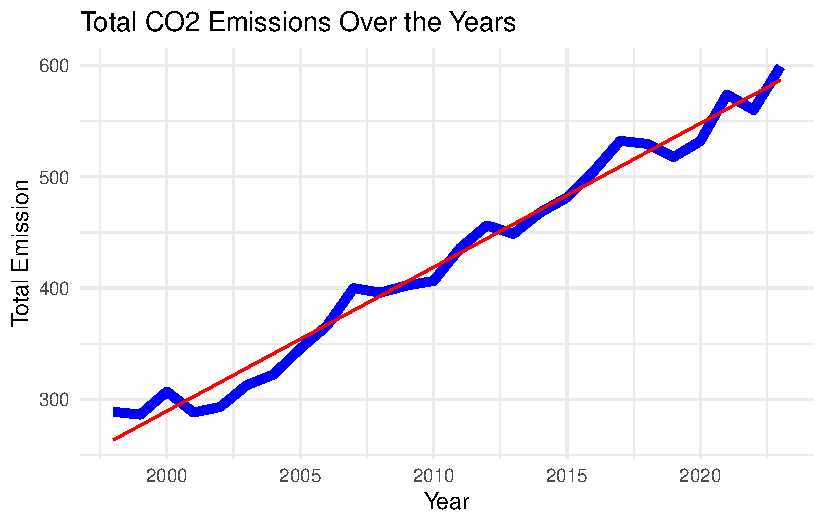
\includegraphics{project_files/figure-pdf/unnamed-chunk-17-1.pdf}

We observe that the industrial sector is the largest consumer of
electricity. The residential and commercial sectors also have high
levels of electricity consumption. In recent years, with the increasing
use of electric vehicles, small increases have been observed in the
transportation sector. In contrast, almost no increase has been seen in
the agriculture and fisheries sectors. The low electricity consumption
in these two sectors despite population growth may indicate a decline in
their operational capacity.

\begin{Shaded}
\begin{Highlighting}[]
\FunctionTok{library}\NormalTok{(ggplot2)}
\FunctionTok{library}\NormalTok{(ggrepel)}
\FunctionTok{library}\NormalTok{(ggthemes)}
\FunctionTok{library}\NormalTok{(moderndive)}

\NormalTok{Co2\_emissions\_by\_sector }\SpecialCharTok{|\textgreater{}}  \FunctionTok{ggplot}\NormalTok{(}\FunctionTok{aes}\NormalTok{(}\AttributeTok{x=}\NormalTok{Year, }\AttributeTok{y=}\NormalTok{Value, }\AttributeTok{color=}\StringTok{\textasciigrave{}}\AttributeTok{CO2 emissions by sector}\StringTok{\textasciigrave{}}\NormalTok{)) }\SpecialCharTok{+} \FunctionTok{geom\_point}\NormalTok{(}\AttributeTok{alpha=}\FloatTok{0.5}\NormalTok{, }\AttributeTok{position =} \FunctionTok{position\_jitter}\NormalTok{()) }\SpecialCharTok{+} \FunctionTok{ylab}\NormalTok{(}\StringTok{"Value of Co2 emissions"}\NormalTok{) }\SpecialCharTok{+} \FunctionTok{ggtitle}\NormalTok{(}\StringTok{"CO2 Emissions by Sector Over the Years"}\NormalTok{) }\SpecialCharTok{+} \FunctionTok{theme\_hc}\NormalTok{(}\AttributeTok{base\_size =} \DecValTok{5}\NormalTok{) }\SpecialCharTok{+} \FunctionTok{theme}\NormalTok{(}\AttributeTok{legend.position =}\StringTok{"none"}\NormalTok{, }\AttributeTok{legend.text =} \FunctionTok{element\_text}\NormalTok{(}\AttributeTok{size=}\DecValTok{5}\NormalTok{), }\AttributeTok{strip.text =} \FunctionTok{element\_text}\NormalTok{(}\AttributeTok{size=}\DecValTok{7}\NormalTok{)) }\SpecialCharTok{+} \FunctionTok{facet\_wrap}\NormalTok{(}\SpecialCharTok{\textasciitilde{}}\StringTok{\textasciigrave{}}\AttributeTok{CO2 emissions by sector}\StringTok{\textasciigrave{}}\NormalTok{, }\AttributeTok{ncol=}\DecValTok{3}\NormalTok{) }\SpecialCharTok{+} \FunctionTok{geom\_smooth}\NormalTok{(}\AttributeTok{method=}\StringTok{"lm"}\NormalTok{, }\AttributeTok{se=}\ConstantTok{FALSE}\NormalTok{,}\AttributeTok{alpha=}\FloatTok{0.3}\NormalTok{)}
\end{Highlighting}
\end{Shaded}

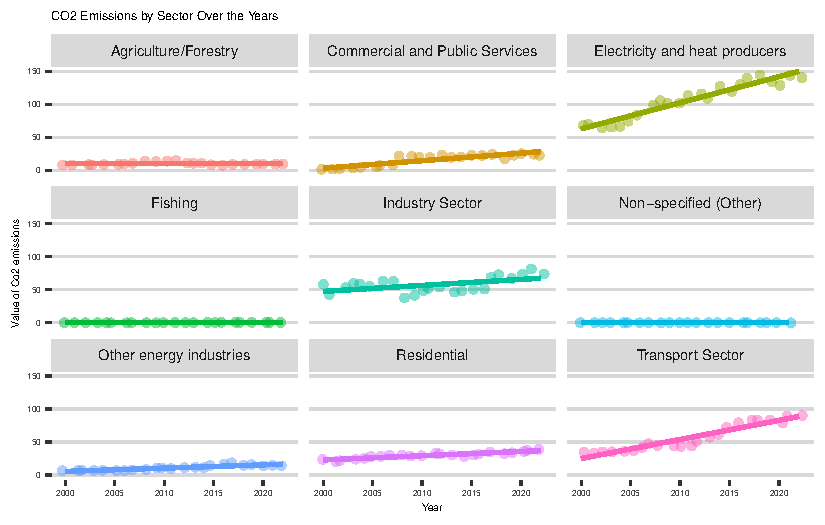
\includegraphics{project_files/figure-pdf/unnamed-chunk-18-1.pdf}

\begin{Shaded}
\begin{Highlighting}[]
\NormalTok{master\_data }\OtherTok{\textless{}{-}}\NormalTok{ master\_data }\SpecialCharTok{|\textgreater{}} \FunctionTok{filter}\NormalTok{(}\SpecialCharTok{!}\FunctionTok{is.na}\NormalTok{(}\StringTok{\textasciigrave{}}\AttributeTok{CO2 emissions per capita}\StringTok{\textasciigrave{}}\NormalTok{))}

\FunctionTok{ggplot}\NormalTok{(master\_data,}\FunctionTok{aes}\NormalTok{(}\AttributeTok{x =}\NormalTok{ Year, }\AttributeTok{y =} \StringTok{\textasciigrave{}}\AttributeTok{CO2 emissions per capita}\StringTok{\textasciigrave{}}\NormalTok{)) }\SpecialCharTok{+}
  \FunctionTok{geom\_line}\NormalTok{(}\AttributeTok{color =} \StringTok{"darkred"}\NormalTok{) }\SpecialCharTok{+}
  \FunctionTok{labs}\NormalTok{(}\AttributeTok{title =} \StringTok{"CO2 Emissions Per Capita (tCO2)"}\NormalTok{, }\AttributeTok{x =} \StringTok{"Year"}\NormalTok{, }\AttributeTok{y =} \StringTok{"tCO2"}\NormalTok{) }\SpecialCharTok{+}
  \FunctionTok{theme\_calc}\NormalTok{()}
\end{Highlighting}
\end{Shaded}

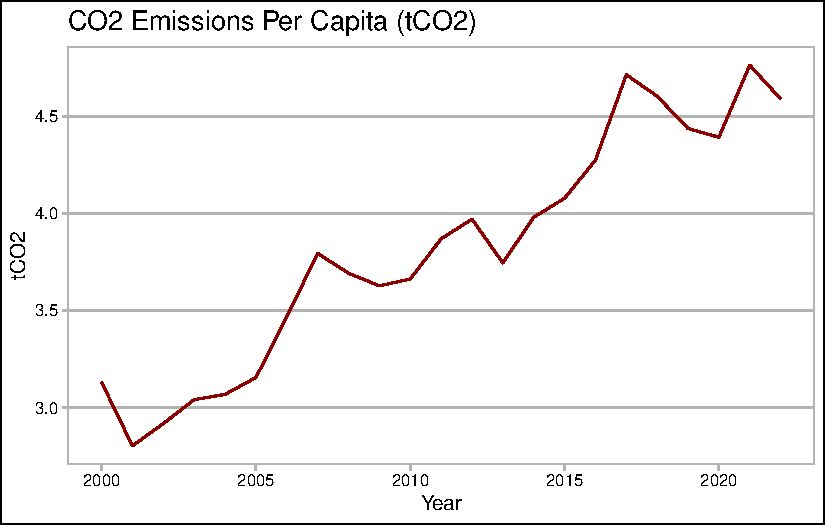
\includegraphics{project_files/figure-pdf/unnamed-chunk-19-1.pdf}

The annual distribution of energy sources used for electricity
generation has changed as follows:

\begin{Shaded}
\begin{Highlighting}[]
\FunctionTok{library}\NormalTok{(dplyr)}
\FunctionTok{library}\NormalTok{(tidyr)}
\FunctionTok{library}\NormalTok{(ggplot2)}
\FunctionTok{library}\NormalTok{(ggstream)}
\FunctionTok{library}\NormalTok{(streamgraph)}
\FunctionTok{library}\NormalTok{(plotly)}


\FunctionTok{colnames}\NormalTok{(total\_energy\_supply) }\OtherTok{\textless{}{-}} \FunctionTok{c}\NormalTok{(}\StringTok{"Sector"}\NormalTok{, }\StringTok{"Value"}\NormalTok{, }\StringTok{"Year"}\NormalTok{)}

\NormalTok{aa }\OtherTok{\textless{}{-}} \FunctionTok{plot\_ly}\NormalTok{(total\_energy\_supply, }\AttributeTok{x =} \SpecialCharTok{\textasciitilde{}}\NormalTok{Sector, }\AttributeTok{y=}\SpecialCharTok{\textasciitilde{}}\NormalTok{Value, }\AttributeTok{frame=}\SpecialCharTok{\textasciitilde{}}\NormalTok{Year, }\AttributeTok{color=}\SpecialCharTok{\textasciitilde{}}\NormalTok{Sector)}
\NormalTok{aa}
\end{Highlighting}
\end{Shaded}

The percentage change in emissions by sector is as follows:

\begin{Shaded}
\begin{Highlighting}[]
\NormalTok{emissions\_by\_sector }\OtherTok{\textless{}{-}}\NormalTok{master\_data }\SpecialCharTok{|\textgreater{}} \FunctionTok{group\_by}\NormalTok{(Year) }\SpecialCharTok{|\textgreater{}} \FunctionTok{pivot\_longer}\NormalTok{(}\AttributeTok{cols =}\NormalTok{ Energy}\SpecialCharTok{:}\NormalTok{Waste,}
                            \AttributeTok{names\_to =} \StringTok{"Emissions\_sector"}\NormalTok{,}
                            \AttributeTok{values\_to =} \StringTok{"Value"}\NormalTok{) }\SpecialCharTok{|\textgreater{}} \FunctionTok{mutate}\NormalTok{(}\AttributeTok{Percentage =}\NormalTok{ Value}\SpecialCharTok{/}\FunctionTok{sum}\NormalTok{(Value)}\SpecialCharTok{*}\DecValTok{100}\NormalTok{)}

\FunctionTok{plot\_ly}\NormalTok{(emissions\_by\_sector,}
        \AttributeTok{labels =} \SpecialCharTok{\textasciitilde{}}\NormalTok{Emissions\_sector,}
        \AttributeTok{values =} \SpecialCharTok{\textasciitilde{}}\NormalTok{Value,}
        \AttributeTok{frame =} \SpecialCharTok{\textasciitilde{}}\NormalTok{Year,}
        \AttributeTok{type =} \StringTok{\textquotesingle{}pie\textquotesingle{}}\NormalTok{,}
        \AttributeTok{textinfo =} \StringTok{\textquotesingle{}percent\textquotesingle{}}\NormalTok{,}
        \AttributeTok{insidetextorientation =} \StringTok{\textquotesingle{}radial\textquotesingle{}}\NormalTok{) }
\end{Highlighting}
\end{Shaded}

Strong correlation results have shown that as the population increases,
CO₂ emissions from fuel sources also rise. Additionally, as per capita
electricity consumption increases, per capita CO₂ emissions also
increase. A strong positive relationship has been observed between
electricity generation and economic growth (GDP).\\
The share of renewable energy sources has not shown a directly negative
relationship with other variables in the system at this stage. This may
be due to its relatively low share in total energy usage.

\begin{Shaded}
\begin{Highlighting}[]
\FunctionTok{library}\NormalTok{(ggcorrplot)}
\NormalTok{veri }\OtherTok{\textless{}{-}}\NormalTok{ master\_data[,}\FunctionTok{c}\NormalTok{(}\StringTok{"mid\_year\_population"}\NormalTok{,}
                      \StringTok{"value\_usd"}\NormalTok{,}
                      \StringTok{"CO2 emissions from fuel combustion"}\NormalTok{,}
                      \StringTok{"CO2 emissions per capita"}\NormalTok{,}
                      \StringTok{"Electricity consumption per capita (MWh)"}\NormalTok{,}
                      \StringTok{"Total electricity production (GWh)"}\NormalTok{,}
                      \StringTok{"Modern renewables(\%)"}\NormalTok{,}
                      \StringTok{"Renewables share of electricity generation (\%)"}\NormalTok{)] }

\NormalTok{core\_1 }\OtherTok{\textless{}{-}}\FunctionTok{cor}\NormalTok{(veri, }\AttributeTok{use=}\StringTok{"complete.obs"}\NormalTok{)}



\NormalTok{kisaltma }\OtherTok{\textless{}{-}} \FunctionTok{c}\NormalTok{(}\StringTok{"Population"}\NormalTok{,}\StringTok{"GDP"}\NormalTok{,}\StringTok{"CO2 From Fuel"}\NormalTok{,}\StringTok{"CO2 Per Capita"}\NormalTok{,}\StringTok{"Electricity Use Per Capita"}\NormalTok{, }\StringTok{"Electricity Production Total"}\NormalTok{,}\StringTok{"Modern RE Share Final Energy"}\NormalTok{,}\StringTok{"Renewables Share Electricity"}\NormalTok{)}

\FunctionTok{colnames}\NormalTok{(core\_1) }\OtherTok{\textless{}{-}}\NormalTok{ kisaltma}
\FunctionTok{rownames}\NormalTok{(core\_1) }\OtherTok{\textless{}{-}}\NormalTok{ kisaltma}

\FunctionTok{ggcorrplot}\NormalTok{(core\_1,}\AttributeTok{lab=}\NormalTok{T,}\AttributeTok{lab\_size=}\DecValTok{3}\NormalTok{,}\AttributeTok{type=}\StringTok{"lower"}\NormalTok{,}\AttributeTok{tl.cex=}\DecValTok{8}\NormalTok{,}\AttributeTok{tl.srt=}\DecValTok{45}\NormalTok{) }
\end{Highlighting}
\end{Shaded}

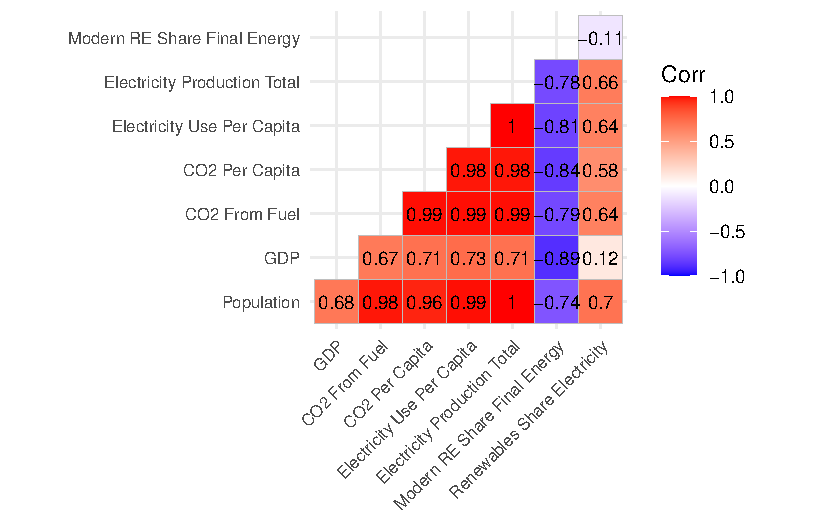
\includegraphics{project_files/figure-pdf/unnamed-chunk-22-1.pdf}

The heatmap below shows the correlations between per capita CO₂
emissions and electricity generation sources. The graph indicates a very
high correlation coefficient between coal and CO₂ emissions, suggesting
that coal use in electricity production is one of the main contributors
to the increase in emissions. Renewable sources such as wind,
geothermal, and hydro also show a positive correlation. However, this
may not be due to their direct contribution to emissions, but rather
because their increasing share in electricity production coincides with
an overall rise in total generation and emissions. A negative
correlation is observed for oil (r = --0.88). Since oil has a relatively
small share in electricity production, its reduction has little effect
on decreasing total emissions.

\begin{Shaded}
\begin{Highlighting}[]
\FunctionTok{library}\NormalTok{(dplyr)}
\FunctionTok{library}\NormalTok{(ggplot2)}
\FunctionTok{library}\NormalTok{(tibble)}

\NormalTok{co2 }\OtherTok{\textless{}{-}}\NormalTok{ Co2\_emissions\_per\_cap}
\NormalTok{elec }\OtherTok{\textless{}{-}}\NormalTok{ electricity\_generation\_sources}

\NormalTok{elec\_wide }\OtherTok{\textless{}{-}}\NormalTok{ elec }\SpecialCharTok{|\textgreater{}}
  \FunctionTok{pivot\_wider}\NormalTok{(}\AttributeTok{names\_from =} \StringTok{\textasciigrave{}}\AttributeTok{Electricity generation sources (GWh)}\StringTok{\textasciigrave{}}\NormalTok{,}
              \AttributeTok{values\_from =}\NormalTok{ Value)}

\CommentTok{\# Verileri yıl üzerinden birleştir}
\NormalTok{yil\_ortakli\_2 }\OtherTok{\textless{}{-}} \FunctionTok{left\_join}\NormalTok{(co2, elec\_wide, }\AttributeTok{by =} \StringTok{"Year"}\NormalTok{)}

\NormalTok{core\_2 }\OtherTok{\textless{}{-}}\NormalTok{ yil\_ortakli\_2 }\SpecialCharTok{\%\textgreater{}\%}
  \FunctionTok{select}\NormalTok{(}\StringTok{\textasciigrave{}}\AttributeTok{CO2 emissions per capita}\StringTok{\textasciigrave{}}\NormalTok{, Coal, }\StringTok{\textasciigrave{}}\AttributeTok{Natural gas}\StringTok{\textasciigrave{}}\NormalTok{, Oil, Hydro, Wind, Geothermal) }\SpecialCharTok{\%\textgreater{}\%}
  \FunctionTok{mutate}\NormalTok{(}\FunctionTok{across}\NormalTok{(}\FunctionTok{everything}\NormalTok{(), as.numeric))}

\NormalTok{kore\_matris }\OtherTok{\textless{}{-}} \FunctionTok{cor}\NormalTok{(core\_2, }\AttributeTok{use =} \StringTok{"complete.obs"}\NormalTok{)}

\NormalTok{corr }\OtherTok{\textless{}{-}} \FunctionTok{as.data.frame}\NormalTok{(kore\_matris[, }\StringTok{"CO2 emissions per capita"}\NormalTok{])}
\NormalTok{corr }\OtherTok{\textless{}{-}} \FunctionTok{rownames\_to\_column}\NormalTok{(corr, }\AttributeTok{var =} \StringTok{"Source"}\NormalTok{)}
\FunctionTok{colnames}\NormalTok{(corr)[}\DecValTok{2}\NormalTok{] }\OtherTok{\textless{}{-}} \StringTok{"Correlation"}


\NormalTok{corr }\OtherTok{\textless{}{-}}\NormalTok{ corr }\SpecialCharTok{\%\textgreater{}\%} \FunctionTok{filter}\NormalTok{(Source }\SpecialCharTok{!=} \StringTok{"CO2\_per\_capita"}\NormalTok{) }\CommentTok{\#kendiyle kıyası kaldırdık}

\FunctionTok{ggplot}\NormalTok{(corr, }\FunctionTok{aes}\NormalTok{(}\AttributeTok{x =} \StringTok{"CO2\_per\_capita"}\NormalTok{, }\AttributeTok{y =} \FunctionTok{reorder}\NormalTok{(Source, Correlation), }\AttributeTok{fill =}\NormalTok{ Correlation)) }\SpecialCharTok{+}
  \FunctionTok{geom\_tile}\NormalTok{(}\AttributeTok{width =} \FloatTok{0.5}\NormalTok{) }\SpecialCharTok{+}
  \FunctionTok{geom\_text}\NormalTok{(}\FunctionTok{aes}\NormalTok{(}\AttributeTok{label =} \FunctionTok{round}\NormalTok{(Correlation, }\DecValTok{2}\NormalTok{)), }\AttributeTok{color =} \StringTok{"white"}\NormalTok{, }\AttributeTok{size =} \DecValTok{4}\NormalTok{) }\SpecialCharTok{+}
  \FunctionTok{scale\_fill\_gradient2}\NormalTok{(}\AttributeTok{low =} \StringTok{"blue"}\NormalTok{, }\AttributeTok{high =} \StringTok{"red"}\NormalTok{, }\AttributeTok{mid =} \StringTok{"white"}\NormalTok{, }\AttributeTok{midpoint =} \DecValTok{0}\NormalTok{) }\SpecialCharTok{+}
  \FunctionTok{labs}\NormalTok{(}\AttributeTok{title =} \StringTok{"Correlation of CO2 Emissions and Electricity Production Sources"}\NormalTok{,}
       \AttributeTok{x =} \StringTok{""}\NormalTok{, }\AttributeTok{y =} \StringTok{"Reosource"}\NormalTok{) }\SpecialCharTok{+}
  \FunctionTok{theme\_minimal}\NormalTok{() }\SpecialCharTok{+}
  \FunctionTok{theme}\NormalTok{(}\AttributeTok{axis.text.x =} \FunctionTok{element\_blank}\NormalTok{(),}
        \AttributeTok{axis.ticks.x =} \FunctionTok{element\_blank}\NormalTok{(),}
        \AttributeTok{axis.title.x =} \FunctionTok{element\_text}\NormalTok{(}\AttributeTok{margin =} \FunctionTok{margin}\NormalTok{(}\AttributeTok{t =} \DecValTok{10}\NormalTok{)), }
        \AttributeTok{axis.title.y =} \FunctionTok{element\_text}\NormalTok{(}\AttributeTok{margin =} \FunctionTok{margin}\NormalTok{(}\AttributeTok{r =} \DecValTok{10}\NormalTok{)),}
        \AttributeTok{plot.title =} \FunctionTok{element\_text}\NormalTok{(}\AttributeTok{size =} \DecValTok{11}
\NormalTok{                                  , }\AttributeTok{face =} \StringTok{"bold"}\NormalTok{))}
\end{Highlighting}
\end{Shaded}

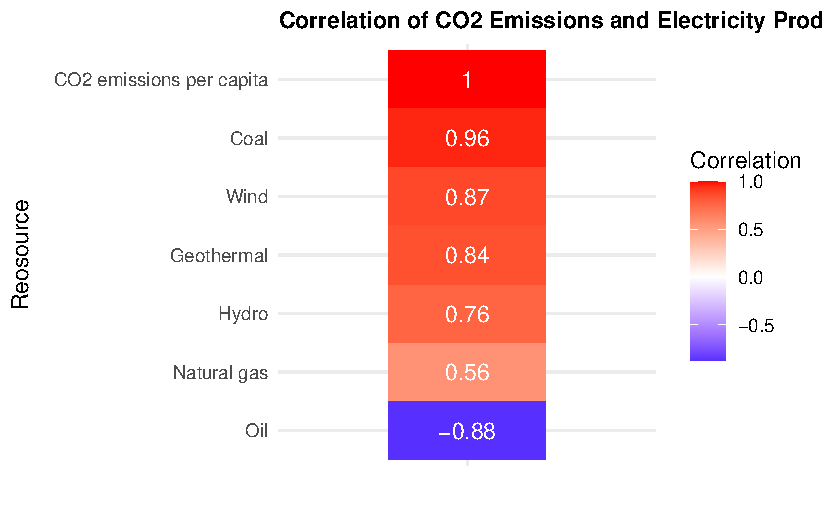
\includegraphics{project_files/figure-pdf/unnamed-chunk-23-1.pdf}

\subsection{3.2 Trend Analysis}\label{trend-analysis}

As electricity consumption per capita increases, carbon emissions also
rise in a strong and statistically significant manner. Specifically, for
each 1 MWh increase in per capita electricity consumption, carbon
emissions increase by approximately 0.92 units.

\begin{Shaded}
\begin{Highlighting}[]
\FunctionTok{library}\NormalTok{(broom)}
\FunctionTok{library}\NormalTok{(dplyr)}
\FunctionTok{library}\NormalTok{(ggplot2)}

\NormalTok{regres\_1 }\OtherTok{\textless{}{-}} \FunctionTok{lm}\NormalTok{(}\StringTok{\textasciigrave{}}\AttributeTok{CO2 emissions per capita}\StringTok{\textasciigrave{}} \SpecialCharTok{\textasciitilde{}} \StringTok{\textasciigrave{}}\AttributeTok{Electricity consumption per capita (MWh)}\StringTok{\textasciigrave{}}\NormalTok{, }\AttributeTok{data=}\NormalTok{master\_data)}
\FunctionTok{summary}\NormalTok{(regres\_1)}
\end{Highlighting}
\end{Shaded}

\begin{verbatim}

Call:
lm(formula = `CO2 emissions per capita` ~ `Electricity consumption per capita (MWh)`, 
    data = master_data)

Residuals:
     Min       1Q   Median       3Q      Max 
-0.21830 -0.08504 -0.01996  0.04434  0.27805 

Coefficients:
                                           Estimate Std. Error t value Pr(>|t|)
(Intercept)                                 1.44127    0.10439   13.81 5.27e-12
`Electricity consumption per capita (MWh)`  0.91777    0.03919   23.42  < 2e-16
                                              
(Intercept)                                ***
`Electricity consumption per capita (MWh)` ***
---
Signif. codes:  0 '***' 0.001 '**' 0.01 '*' 0.05 '.' 0.1 ' ' 1

Residual standard error: 0.119 on 21 degrees of freedom
Multiple R-squared:  0.9631,    Adjusted R-squared:  0.9614 
F-statistic: 548.5 on 1 and 21 DF,  p-value: < 2.2e-16
\end{verbatim}

\begin{Shaded}
\begin{Highlighting}[]
\FunctionTok{tidy}\NormalTok{(regres\_1)}
\end{Highlighting}
\end{Shaded}

\begin{verbatim}
# A tibble: 2 x 5
  term                                     estimate std.error statistic  p.value
  <chr>                                       <dbl>     <dbl>     <dbl>    <dbl>
1 (Intercept)                                 1.44     0.104       13.8 5.27e-12
2 `Electricity consumption per capita (MW~    0.918    0.0392      23.4 1.56e-16
\end{verbatim}

\begin{Shaded}
\begin{Highlighting}[]
\NormalTok{regres\_1 }\SpecialCharTok{|\textgreater{}} \FunctionTok{glance}\NormalTok{() }\SpecialCharTok{|\textgreater{}} \FunctionTok{pull}\NormalTok{(r.squared)}
\end{Highlighting}
\end{Shaded}

\begin{verbatim}
[1] 0.9631286
\end{verbatim}

\begin{Shaded}
\begin{Highlighting}[]
\NormalTok{regres\_1 }\SpecialCharTok{|\textgreater{}} \FunctionTok{glance}\NormalTok{() }\SpecialCharTok{|\textgreater{}} \FunctionTok{pull}\NormalTok{(sigma)}
\end{Highlighting}
\end{Shaded}

\begin{verbatim}
[1] 0.1190368
\end{verbatim}

\begin{Shaded}
\begin{Highlighting}[]
\NormalTok{explanatory\_data }\OtherTok{\textless{}{-}} \FunctionTok{tibble}\NormalTok{(}\StringTok{\textasciigrave{}}\AttributeTok{Electricity consumption per capita (MWh)}\StringTok{\textasciigrave{}}\OtherTok{=} \FunctionTok{c}\NormalTok{(}\FloatTok{1.3}\NormalTok{, }\FloatTok{1.5}\NormalTok{,}\DecValTok{2}\NormalTok{,}\FloatTok{3.5}\NormalTok{,}\FloatTok{3.7}\NormalTok{,}\DecValTok{4}\NormalTok{))}
\FunctionTok{predict}\NormalTok{(regres\_1,explanatory\_data)}
\end{Highlighting}
\end{Shaded}

\begin{verbatim}
       1        2        3        4        5        6 
2.634369 2.817923 3.276806 4.653457 4.837010 5.112340 
\end{verbatim}

\begin{Shaded}
\begin{Highlighting}[]
\NormalTok{prediction\_data }\OtherTok{\textless{}{-}}\NormalTok{ explanatory\_data }\SpecialCharTok{|\textgreater{}} \FunctionTok{mutate}\NormalTok{(}
  \StringTok{\textasciigrave{}}\AttributeTok{CO2 emissions per capita}\StringTok{\textasciigrave{}} \OtherTok{=} \FunctionTok{predict}\NormalTok{(regres\_1,explanatory\_data ))}

\FunctionTok{ggplot}\NormalTok{(master\_data, }\FunctionTok{aes}\NormalTok{(}\AttributeTok{x =} \StringTok{\textasciigrave{}}\AttributeTok{Electricity consumption per capita (MWh)}\StringTok{\textasciigrave{}}\NormalTok{, }\AttributeTok{y=}\StringTok{\textasciigrave{}}\AttributeTok{CO2 emissions per capita}\StringTok{\textasciigrave{}}\NormalTok{)) }\SpecialCharTok{+}
  \FunctionTok{geom\_point}\NormalTok{() }\SpecialCharTok{+}
  \FunctionTok{geom\_smooth}\NormalTok{(}\AttributeTok{method=}\StringTok{"lm"}\NormalTok{) }\SpecialCharTok{+} \FunctionTok{geom\_point}\NormalTok{(}\AttributeTok{data=}\NormalTok{prediction\_data, }\AttributeTok{shape=}\DecValTok{15}\NormalTok{, }\AttributeTok{size=}\DecValTok{2}\NormalTok{,}\AttributeTok{color=}\StringTok{"red"}\NormalTok{)}
\end{Highlighting}
\end{Shaded}

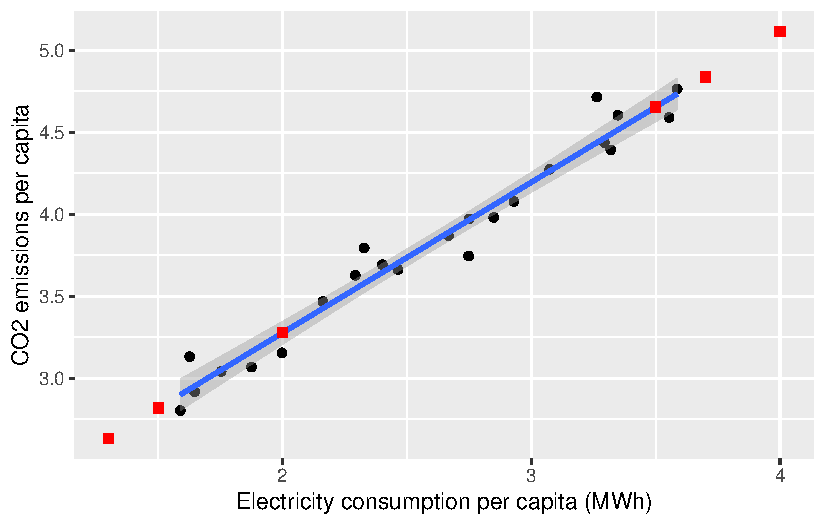
\includegraphics{project_files/figure-pdf/unnamed-chunk-24-1.pdf}

CO₂ emissions are primarily explained by electricity production and the
share of renewable energy. Since GDP was found to have no significant
effect, it was excluded from the analysis.

\begin{Shaded}
\begin{Highlighting}[]
\NormalTok{master\_data }\OtherTok{\textless{}{-}}\NormalTok{ master\_data }\SpecialCharTok{|\textgreater{}} \FunctionTok{mutate}\NormalTok{(}\AttributeTok{gross\_domestic =}\NormalTok{ value\_usd}\SpecialCharTok{*}\NormalTok{mid\_year\_population)}
\NormalTok{lin\_reg\_2 }\OtherTok{=} \FunctionTok{lm}\NormalTok{(Total.x }\SpecialCharTok{\textasciitilde{}} \StringTok{\textasciigrave{}}\AttributeTok{Total electricity production (GWh)}\StringTok{\textasciigrave{}}\SpecialCharTok{+}\StringTok{\textasciigrave{}}\AttributeTok{Renewables share of electricity generation (\%)}\StringTok{\textasciigrave{}}\SpecialCharTok{+}\NormalTok{ gross\_domestic, }\AttributeTok{data=}\NormalTok{master\_data)}

\FunctionTok{summary}\NormalTok{(lin\_reg\_2)}
\end{Highlighting}
\end{Shaded}

\begin{verbatim}

Call:
lm(formula = Total.x ~ `Total electricity production (GWh)` + 
    `Renewables share of electricity generation (%)` + gross_domestic, 
    data = master_data)

Residuals:
    Min      1Q  Median      3Q     Max 
-7.3985 -5.5831 -0.3761  3.9333 13.3644 

Coefficients:
                                                   Estimate Std. Error t value
(Intercept)                                       1.425e+02  6.280e+00  22.688
`Total electricity production (GWh)`              1.357e-03  6.038e-05  22.468
`Renewables share of electricity generation (%)` -8.177e-01  3.418e-01  -2.393
gross_domestic                                    7.359e-09  1.296e-08   0.568
                                                 Pr(>|t|)    
(Intercept)                                      3.18e-15 ***
`Total electricity production (GWh)`             3.80e-15 ***
`Renewables share of electricity generation (%)`   0.0272 *  
gross_domestic                                     0.5769    
---
Signif. codes:  0 '***' 0.001 '**' 0.01 '*' 0.05 '.' 0.1 ' ' 1

Residual standard error: 6.418 on 19 degrees of freedom
Multiple R-squared:  0.9957,    Adjusted R-squared:  0.995 
F-statistic:  1459 on 3 and 19 DF,  p-value: < 2.2e-16
\end{verbatim}

Since multiple regression analysis showed that carbon emissions can be
accurately explained by total electricity production and the share of
renewable energy sources in electricity generation, the analysis was
carried out using this linear model. The model explains 99\% of the
variation in the data (R-squared), and its very low p-value indicates
strong statistical significance.

In terms of relationships:

A 1\% increase in the share of renewable energy in electricity
generation leads to an average decrease of 0.94 units in carbon
emissions, while each 1 GWh increase in total electricity production
results in an average increase of 0.001 units in carbon emissions.

\begin{Shaded}
\begin{Highlighting}[]
\FunctionTok{library}\NormalTok{(broom)}
\FunctionTok{library}\NormalTok{(dplyr)}
\NormalTok{regres\_1 }\OtherTok{\textless{}{-}} \FunctionTok{lm}\NormalTok{(Total.x }\SpecialCharTok{\textasciitilde{}} \StringTok{\textasciigrave{}}\AttributeTok{Total electricity production (GWh)}\StringTok{\textasciigrave{}}\SpecialCharTok{+}\StringTok{\textasciigrave{}}\AttributeTok{Renewables share of electricity generation (\%)}\StringTok{\textasciigrave{}}\NormalTok{ ,}\AttributeTok{data=}\NormalTok{master\_data) }\SpecialCharTok{|\textgreater{}} \FunctionTok{na.omit}\NormalTok{()}
\FunctionTok{summary}\NormalTok{(regres\_1)}
\end{Highlighting}
\end{Shaded}

\begin{verbatim}

Call:
lm(formula = Total.x ~ `Total electricity production (GWh)` + 
    `Renewables share of electricity generation (%)`, data = master_data)

Residuals:
    Min      1Q  Median      3Q     Max 
-7.5851 -5.8446 -0.9368  3.9378 13.0079 

Coefficients:
                                                   Estimate Std. Error t value
(Intercept)                                       1.442e+02  5.460e+00  26.401
`Total electricity production (GWh)`              1.387e-03  2.754e-05  50.360
`Renewables share of electricity generation (%)` -9.417e-01  2.582e-01  -3.647
                                                 Pr(>|t|)    
(Intercept)                                        <2e-16 ***
`Total electricity production (GWh)`               <2e-16 ***
`Renewables share of electricity generation (%)`   0.0016 ** 
---
Signif. codes:  0 '***' 0.001 '**' 0.01 '*' 0.05 '.' 0.1 ' ' 1

Residual standard error: 6.308 on 20 degrees of freedom
Multiple R-squared:  0.9956,    Adjusted R-squared:  0.9952 
F-statistic:  2265 on 2 and 20 DF,  p-value: < 2.2e-16
\end{verbatim}

\begin{Shaded}
\begin{Highlighting}[]
\FunctionTok{tidy}\NormalTok{(regres\_1)}
\end{Highlighting}
\end{Shaded}

\begin{verbatim}
# A tibble: 3 x 5
  term                                     estimate std.error statistic  p.value
  <chr>                                       <dbl>     <dbl>     <dbl>    <dbl>
1 (Intercept)                               1.44e+2 5.46          26.4  5.09e-17
2 `Total electricity production (GWh)`      1.39e-3 0.0000275     50.4  1.52e-22
3 `Renewables share of electricity genera~ -9.42e-1 0.258         -3.65 1.60e- 3
\end{verbatim}

\begin{Shaded}
\begin{Highlighting}[]
\NormalTok{regres\_1 }\SpecialCharTok{|\textgreater{}} \FunctionTok{glance}\NormalTok{() }\SpecialCharTok{|\textgreater{}} \FunctionTok{pull}\NormalTok{(r.squared)}
\end{Highlighting}
\end{Shaded}

\begin{verbatim}
[1] 0.9956048
\end{verbatim}

\begin{Shaded}
\begin{Highlighting}[]
\NormalTok{regres\_1 }\SpecialCharTok{|\textgreater{}} \FunctionTok{glance}\NormalTok{() }\SpecialCharTok{|\textgreater{}} \FunctionTok{pull}\NormalTok{(sigma)}
\end{Highlighting}
\end{Shaded}

\begin{verbatim}
[1] 6.308056
\end{verbatim}

\subsection{3.3 Model Fitting}\label{model-fitting}

A time series analysis of carbon emissions was conducted. The model's
coefficient was found to be 11.5, indicating an average annual increase
of 11.5 units in emissions. The model demonstrated strong forecasting
performance (MAPE = 3\%). If the current trend continues, carbon
emissions are expected to reach around 700 units, as shown in the
forecast table.

\begin{Shaded}
\begin{Highlighting}[]
\FunctionTok{library}\NormalTok{(forecast)}
\FunctionTok{library}\NormalTok{(fpp2)}
\NormalTok{emission }\OtherTok{\textless{}{-}}\NormalTok{ master\_data}\SpecialCharTok{$}\NormalTok{Total.x}
\NormalTok{emission\_ts }\OtherTok{\textless{}{-}} \FunctionTok{ts}\NormalTok{(}\AttributeTok{data=}\NormalTok{emission, }\AttributeTok{start =} \FunctionTok{c}\NormalTok{(}\DecValTok{2000}\NormalTok{), }\AttributeTok{frequency =} \DecValTok{1}\NormalTok{)}


\NormalTok{fitting }\OtherTok{\textless{}{-}} \FunctionTok{auto.arima}\NormalTok{(emission\_ts)}

\FunctionTok{checkresiduals}\NormalTok{(fitting)}
\end{Highlighting}
\end{Shaded}

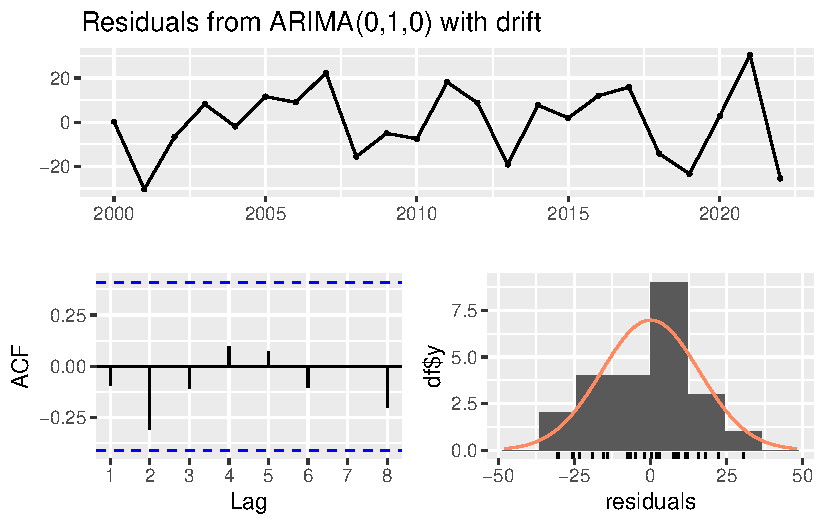
\includegraphics{project_files/figure-pdf/unnamed-chunk-27-1.pdf}

\begin{verbatim}

    Ljung-Box test

data:  Residuals from ARIMA(0,1,0) with drift
Q* = 3.6457, df = 5, p-value = 0.6015

Model df: 0.   Total lags used: 5
\end{verbatim}

\begin{Shaded}
\begin{Highlighting}[]
\FunctionTok{auto.arima}\NormalTok{(emission\_ts)}
\end{Highlighting}
\end{Shaded}

\begin{verbatim}
Series: emission_ts 
ARIMA(0,1,0) with drift 

Coefficients:
        drift
      11.5105
s.e.   3.4128

sigma^2 = 268.4:  log likelihood = -92.22
AIC=188.45   AICc=189.08   BIC=190.63
\end{verbatim}

\begin{Shaded}
\begin{Highlighting}[]
\FunctionTok{summary}\NormalTok{(fitting)}
\end{Highlighting}
\end{Shaded}

\begin{verbatim}
Series: emission_ts 
ARIMA(0,1,0) with drift 

Coefficients:
        drift
      11.5105
s.e.   3.4128

sigma^2 = 268.4:  log likelihood = -92.22
AIC=188.45   AICc=189.08   BIC=190.63

Training set error measures:
                    ME     RMSE      MAE        MPE     MAPE      MASE
Training set 0.0128461 15.65551 12.96707 -0.1260035 3.036878 0.7687117
                    ACF1
Training set -0.09557549
\end{verbatim}

\begin{Shaded}
\begin{Highlighting}[]
\NormalTok{fitting }\SpecialCharTok{|\textgreater{}} \FunctionTok{forecast}\NormalTok{(}\AttributeTok{h=}\DecValTok{15}\NormalTok{) }\SpecialCharTok{|\textgreater{}} \FunctionTok{autoplot}\NormalTok{(}\AttributeTok{color=}\StringTok{"red"}\NormalTok{) }\SpecialCharTok{+} \FunctionTok{theme\_minimal}\NormalTok{()}
\end{Highlighting}
\end{Shaded}

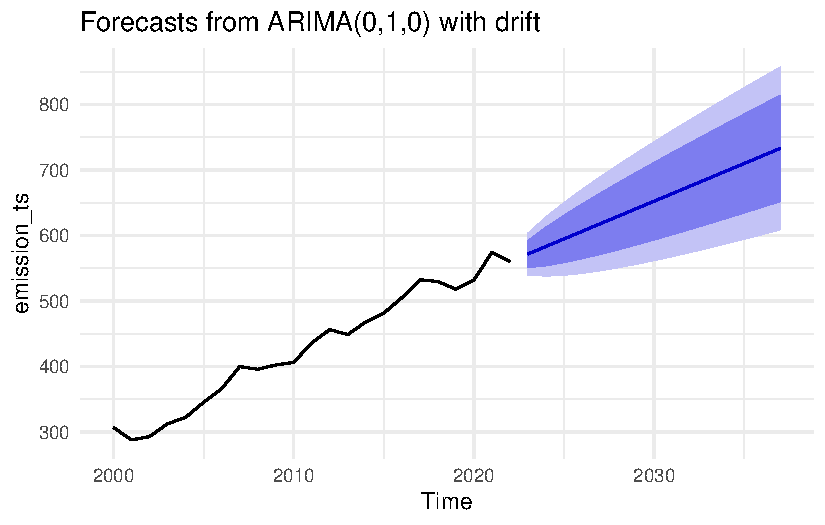
\includegraphics{project_files/figure-pdf/unnamed-chunk-27-2.pdf}

\begin{Shaded}
\begin{Highlighting}[]
\FunctionTok{predict}\NormalTok{(emission\_ts)}
\end{Highlighting}
\end{Shaded}

\begin{verbatim}
     Point Forecast    Lo 80    Hi 80    Lo 95    Hi 95
2023       588.9250 570.5998 607.2502 560.8990 616.9510
2024       602.2172 583.8920 620.5424 574.1912 630.2431
2025       615.5093 597.1841 633.8346 587.4834 643.5353
2026       628.8015 610.4763 647.1267 600.7755 656.8275
2027       642.0937 623.7685 660.4189 614.0677 670.1197
2028       655.3859 637.0607 673.7111 627.3599 683.4119
2029       668.6781 650.3528 687.0033 640.6521 696.7041
2030       681.9702 663.6450 700.2955 653.9442 709.9962
2031       695.2624 676.9372 713.5876 667.2364 723.2884
2032       708.5546 690.2294 726.8798 680.5286 736.5806
\end{verbatim}

The structure of emission changes based on electricity production has
been analyzed. This change depends on the scenario of external factors,
particularly the amount of electricity produced.

\begin{Shaded}
\begin{Highlighting}[]
\FunctionTok{library}\NormalTok{(dplyr)}
\FunctionTok{library}\NormalTok{(ggplot2)}

\NormalTok{total\_electric }\OtherTok{\textless{}{-}}\NormalTok{ master\_data[[}\StringTok{"Total electricity production (GWh)"}\NormalTok{]] }
\NormalTok{electric\_emission }\OtherTok{\textless{}{-}}\NormalTok{ master\_data}\SpecialCharTok{$}\NormalTok{Total.x}
\NormalTok{Emission }\OtherTok{\textless{}{-}} \FunctionTok{ts}\NormalTok{(}\AttributeTok{data=}\NormalTok{electric\_emission, }\AttributeTok{start =} \FunctionTok{c}\NormalTok{(}\DecValTok{2000}\NormalTok{), }\AttributeTok{frequency =} \DecValTok{1}\NormalTok{)}
\NormalTok{fit }\OtherTok{\textless{}{-}} \FunctionTok{auto.arima}\NormalTok{(Emission, }\AttributeTok{xreg =}\NormalTok{ total\_electric)}
\NormalTok{fit}
\end{Highlighting}
\end{Shaded}

\begin{verbatim}
Series: Emission 
Regression with ARIMA(0,0,0) errors 

Coefficients:
      intercept    xreg
       133.4205  0.0013
s.e.     5.5343  0.0002

sigma^2 = 63.1:  log likelihood = -79.25
AIC=164.51   AICc=165.77   BIC=167.91
\end{verbatim}

\begin{Shaded}
\begin{Highlighting}[]
\FunctionTok{checkresiduals}\NormalTok{(fit)}
\end{Highlighting}
\end{Shaded}

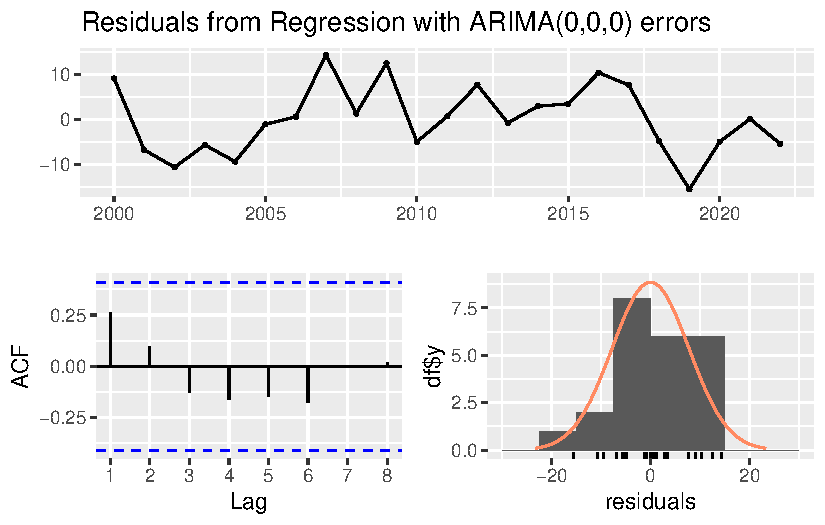
\includegraphics{project_files/figure-pdf/unnamed-chunk-28-1.pdf}

\begin{verbatim}

    Ljung-Box test

data:  Residuals from Regression with ARIMA(0,0,0) errors
Q* = 4.0203, df = 5, p-value = 0.5465

Model df: 0.   Total lags used: 5
\end{verbatim}

\begin{Shaded}
\begin{Highlighting}[]
\NormalTok{future\_electric\_production }\OtherTok{\textless{}{-}} \FunctionTok{c}\NormalTok{(}\DecValTok{330000}\NormalTok{,}\DecValTok{350000}\NormalTok{, }\DecValTok{400000}\NormalTok{, }\DecValTok{350000}\NormalTok{)}
\FunctionTok{forecast}\NormalTok{(fit, }\AttributeTok{xreg =}\NormalTok{ future\_electric\_production) }\SpecialCharTok{|\textgreater{}} \FunctionTok{autoplot}\NormalTok{() }\SpecialCharTok{+} \FunctionTok{theme\_minimal}\NormalTok{()}
\end{Highlighting}
\end{Shaded}

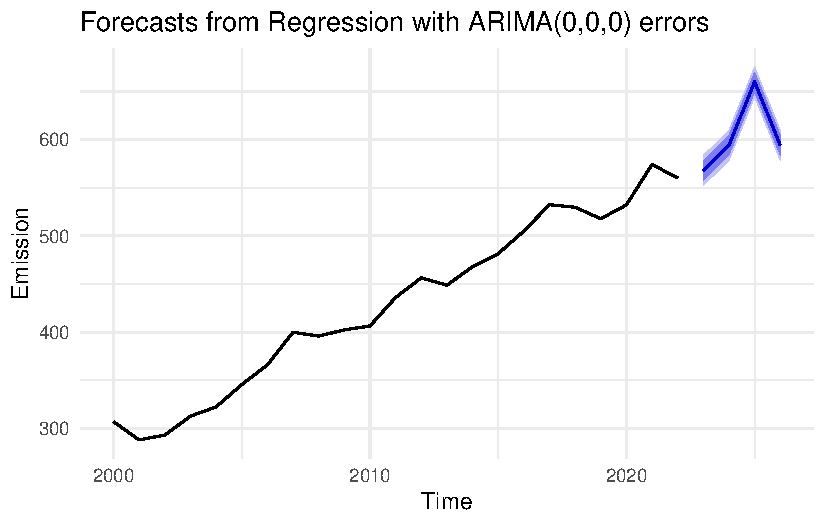
\includegraphics{project_files/figure-pdf/unnamed-chunk-28-2.pdf}

The forecast of carbon emissions was conducted based on the relationship
identified in the previous trend analysis. While carbon emissions were
initially modeled as dependent on these two variables, data for the next
six years were entered, and future carbon emissions were predicted
accordingly.

\begin{Shaded}
\begin{Highlighting}[]
\NormalTok{lin\_reg\_1 }\OtherTok{=} \FunctionTok{lm}\NormalTok{(Total.x }\SpecialCharTok{\textasciitilde{}} \StringTok{\textasciigrave{}}\AttributeTok{Total electricity production (GWh)}\StringTok{\textasciigrave{}}\SpecialCharTok{+}\StringTok{\textasciigrave{}}\AttributeTok{Renewables share of electricity generation (\%)}\StringTok{\textasciigrave{}}\NormalTok{, }\AttributeTok{data=}\NormalTok{master\_data) }\SpecialCharTok{|\textgreater{}} \FunctionTok{na.omit}\NormalTok{()}

\NormalTok{fitted\_values }\OtherTok{\textless{}{-}} \FunctionTok{predict}\NormalTok{(lin\_reg\_1)}

\FunctionTok{length}\NormalTok{(master\_data}\SpecialCharTok{$}\NormalTok{Year)}
\end{Highlighting}
\end{Shaded}

\begin{verbatim}
[1] 23
\end{verbatim}

\begin{Shaded}
\begin{Highlighting}[]
\FunctionTok{length}\NormalTok{(fitted\_values)}
\end{Highlighting}
\end{Shaded}

\begin{verbatim}
[1] 23
\end{verbatim}

\begin{Shaded}
\begin{Highlighting}[]
\NormalTok{future\_data }\OtherTok{\textless{}{-}} \FunctionTok{data.frame}\NormalTok{(}
  \AttributeTok{check.names =} \ConstantTok{FALSE}\NormalTok{,}
  \StringTok{\textasciigrave{}}\AttributeTok{Total electricity production (GWh)}\StringTok{\textasciigrave{}} \OtherTok{=} \FunctionTok{c}\NormalTok{(}\DecValTok{330000}\NormalTok{,}\DecValTok{340000}\NormalTok{, }\DecValTok{350000}\NormalTok{, }\DecValTok{370000}\NormalTok{, }\DecValTok{400000}\NormalTok{,}\DecValTok{450000}\NormalTok{),}
  \StringTok{\textasciigrave{}}\AttributeTok{Renewables share of electricity generation (\%)}\StringTok{\textasciigrave{}} \OtherTok{=} \FunctionTok{c}\NormalTok{(}\DecValTok{35}\NormalTok{, }\DecValTok{38}\NormalTok{, }\DecValTok{40}\NormalTok{, }\DecValTok{43}\NormalTok{, }\DecValTok{45}\NormalTok{,}\DecValTok{50}\NormalTok{)}
\NormalTok{)}
\NormalTok{forecasted\_values }\OtherTok{\textless{}{-}} \FunctionTok{predict}\NormalTok{(lin\_reg\_1, }\AttributeTok{newdata =}\NormalTok{ future\_data)}
\NormalTok{future\_years }\OtherTok{\textless{}{-}} \DecValTok{2023}\SpecialCharTok{:}\DecValTok{2028}

\NormalTok{df\_actual }\OtherTok{\textless{}{-}} \FunctionTok{data.frame}\NormalTok{(}
  \AttributeTok{Year =}\NormalTok{ master\_data}\SpecialCharTok{$}\NormalTok{Year,}
  \AttributeTok{CO2 =}\NormalTok{ master\_data}\SpecialCharTok{$}\NormalTok{Total.x,}
  \AttributeTok{Type =} \StringTok{"Actual"}
\NormalTok{)}

\NormalTok{df\_fitted }\OtherTok{\textless{}{-}} \FunctionTok{data.frame}\NormalTok{(}
  \AttributeTok{Year =}\NormalTok{ master\_data}\SpecialCharTok{$}\NormalTok{Year,}
  \AttributeTok{CO2 =}\NormalTok{ fitted\_values,}
  \AttributeTok{Type =} \StringTok{"Fitted"}
\NormalTok{)}

\NormalTok{df\_forecasted }\OtherTok{\textless{}{-}} \FunctionTok{data.frame}\NormalTok{(}
  \AttributeTok{Year =}\NormalTok{ future\_years,}
  \AttributeTok{CO2 =}\NormalTok{ forecasted\_values,}
  \AttributeTok{Type =} \StringTok{"Forecasted"}
\NormalTok{)}

\CommentTok{\# Hepsini birleştir}
\NormalTok{df\_all }\OtherTok{\textless{}{-}} \FunctionTok{rbind}\NormalTok{(df\_actual, df\_fitted, df\_forecasted)}

\FunctionTok{library}\NormalTok{(ggplot2)}

\FunctionTok{ggplot}\NormalTok{(df\_all, }\FunctionTok{aes}\NormalTok{(}\AttributeTok{x =}\NormalTok{ Year, }\AttributeTok{y =}\NormalTok{ CO2, }\AttributeTok{color =}\NormalTok{ Type, }\AttributeTok{linetype =}\NormalTok{ Type)) }\SpecialCharTok{+}
  \FunctionTok{geom\_line}\NormalTok{(}\AttributeTok{size =} \DecValTok{1}\NormalTok{) }\SpecialCharTok{+}
  \FunctionTok{geom\_point}\NormalTok{(}\AttributeTok{size =} \FloatTok{1.2}\NormalTok{) }\SpecialCharTok{+}
  \FunctionTok{scale\_color\_manual}\NormalTok{(}\AttributeTok{values =} \FunctionTok{c}\NormalTok{(}\StringTok{"Actual"} \OtherTok{=} \StringTok{"black"}\NormalTok{, }\StringTok{"Fitted"} \OtherTok{=} \StringTok{"blue"}\NormalTok{, }\StringTok{"Forecasted"} \OtherTok{=} \StringTok{"red"}\NormalTok{)) }\SpecialCharTok{+}
  \FunctionTok{scale\_linetype\_manual}\NormalTok{(}\AttributeTok{values =} \FunctionTok{c}\NormalTok{(}\StringTok{"Actual"} \OtherTok{=} \StringTok{"solid"}\NormalTok{, }\StringTok{"Fitted"} \OtherTok{=} \StringTok{"dashed"}\NormalTok{, }\StringTok{"Forecasted"} \OtherTok{=} \StringTok{"dotdash"}\NormalTok{)) }\SpecialCharTok{+}
  \FunctionTok{ggtitle}\NormalTok{(}\StringTok{"CO2 Emissions Model Fitting"}\NormalTok{) }\SpecialCharTok{+}
  \FunctionTok{ylab}\NormalTok{(}\StringTok{"CO2 Emissions"}\NormalTok{) }\SpecialCharTok{+} \FunctionTok{xlab}\NormalTok{(}\StringTok{"Year"}\NormalTok{) }\SpecialCharTok{+}
  \FunctionTok{theme\_minimal}\NormalTok{() }\SpecialCharTok{+}
  \FunctionTok{theme}\NormalTok{(}\AttributeTok{plot.title =} \FunctionTok{element\_text}\NormalTok{(}\AttributeTok{size =} \DecValTok{12}\NormalTok{))}
\end{Highlighting}
\end{Shaded}

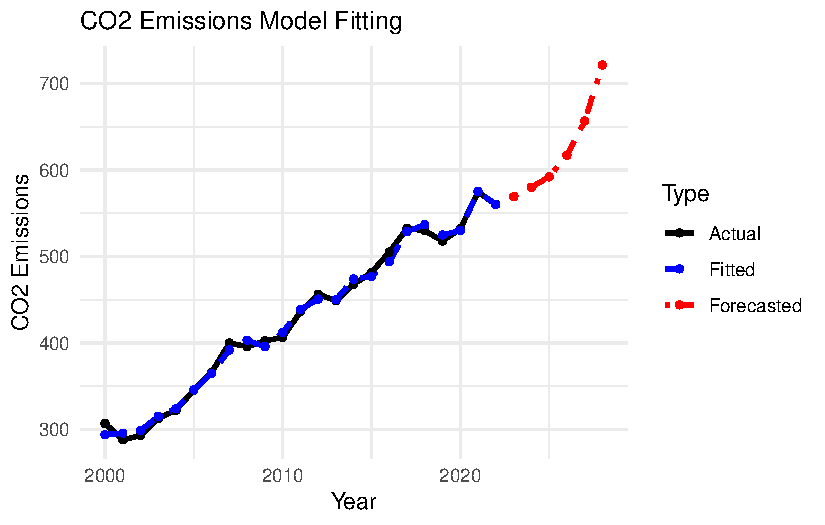
\includegraphics{project_files/figure-pdf/unnamed-chunk-29-1.pdf}

\begin{Shaded}
\begin{Highlighting}[]
\NormalTok{df\_forecasted}
\end{Highlighting}
\end{Shaded}

\begin{verbatim}
  Year      CO2       Type
1 2023 568.8835 Forecasted
2 2024 579.9277 Forecasted
3 2025 591.9137 Forecasted
4 2026 616.8274 Forecasted
5 2027 656.5522 Forecasted
6 2028 721.1908 Forecasted
\end{verbatim}

\subsection{3.4 Results}\label{results}

The analyses conducted within the scope of this study reveal that
between 2000 and 2022, the primary source of CO₂ emissions in Turkey has
been electricity and heat production. The industrial sector stands out
as the largest consumer of electricity, followed by residential and
public services, which also account for significant portions of
consumption. In contrast, electricity use and emissions in the
agriculture and fisheries sectors have remained relatively stable.

Correlation analyses identified very strong positive relationships
between per capita CO₂ emissions and per capita electricity consumption
(r = 0.98), total electricity production (r = 0.94), and overall
emissions. Source-based analysis showed that coal consumption had the
strongest positive correlation with CO₂ emissions (r = 0.96), while
petroleum use was found to have a significant negative correlation (r =
--0.88).

Regression modeling indicated that per capita electricity consumption
was a highly accurate predictor of CO₂ emissions (R² ≈ 0.97). A
multivariate regression model projected that, with continued growth in
production, CO₂ emissions could reach approximately 730 MtCO₂ by 2029.

Although the increasing share of renewable energy is a positive trend,
it has not been sufficient to offset the overall growth in production.
The time series analysis using the ARIMA(0,1,0) with drift model passed
all residual diagnostics and forecasted a steady rise in production over
the next decade. When compared to the ETS model, ARIMA delivered better
performance with lower error margins. Based on the regression analysis
linking total emissions to total electricity production and the share of
renewables, future emission levels were estimated. These findings
clearly indicate that, if current production and consumption patterns
persist, CO₂ emissions are likely to continue rising.

\section{4. Results and Key Takeaways}\label{results-and-key-takeaways}

In our analysis, we examined the relationship between Turkey's
electricity production, the distribution of energy sources, and CO₂
emissions. We defined our data range as the last 20 years and used
exploratory analysis, correlation studies, regression models, and time
series forecasting methods. The key findings are as follows:

Electricity production in Turkey has been continuously increasing, and
the rise in population and demand from the industrial sector has
significantly contributed to the increase in CO₂ emissions.

Additionally, CO₂ emissions are strongly associated with electricity
generation based on fossil fuels, especially coal. Our findings indicate
that coal use in electricity production is still remarkably high in
Turkey.

Although the use of renewable energy sources is growing day by day, this
increase has not been sufficient to offset the rise in total electricity
production and therefore has not had a significant effect on reducing
emissions.

Both regression and time series models show that if current trends
continue, CO₂ emissions will increase sharply in the coming years.

It is not enough to simply invest in clean energy sources. Although such
investments have begun to grow in recent years, no downward trend in CO₂
emissions has been observed. Reducing the use of fossil fuels is
essential.




\end{document}
